% Compiling for Distributed Memory: A Historical Survey and Taxonomy
% Build: cd paper && latexmk -pdf main.tex   (or `make paper` from the repo root)
\documentclass[journal]{IEEEtran}

\usepackage[utf8]{inputenc}
\usepackage[T1]{fontenc}
\usepackage{cite}
\usepackage{graphicx}
\usepackage{booktabs}
\usepackage{array}
\usepackage{amsmath,amssymb}
\usepackage{url}
\usepackage{xcolor}
\usepackage{enumitem}
\usepackage[hidelinks]{hyperref}

\graphicspath{{figures/}}

% ---- evidence-level markup (see docs/methodology.md, Sec. 9) ----------------
% \fact{...}   source-supported statement (must carry a \cite)
% \ours{...}   survey taxonomy / grouping introduced by this paper
% \infer{...}  inference or synthesis; also listed in docs/historical-claims.md
% \todo{...}   incomplete claim or missing evidence
\newcommand{\fact}[1]{#1}
\newcommand{\ours}[1]{#1}
\newcommand{\infer}[1]{#1}
\newcommand{\todo}[1]{\textcolor{red!70!black}{[TODO: #1]}}
\newcommand{\sys}[1]{\textsc{#1}}

\begin{document}

\title{Compiling for Distributed Memory: A Historical Survey and Taxonomy from Global Arrays to Mesh-Sharded AI Systems}

\author{Sameeran~Joshi%
\thanks{Manuscript draft generated from the open catalog at \url{https://github.com/Sameeranjoshi/dist_compilers}. This is a working draft; see the repository ROADMAP for status.}}

\markboth{Draft --- Distributed-Memory Compilers: A Historical Survey and Taxonomy}{}

\maketitle

\begin{abstract}
Compilers that target machines with physically distributed memories must decide where data lives, where computation runs, and what communication connects the two. These decisions were posed as compiler problems in the late 1980s for hypercubes and multicomputers, standardised in High Performance Fortran in the 1990s, largely left to hand-written message passing in the 2000s, and have returned in the 2020s as sharding propagation for accelerator meshes and wafer-scale machines. This article surveys that history with a reproducible method: an operational definition of a distributed-memory compiler, an openly maintained and schema-validated catalog, and a taxonomy on independent axes that separates the decision procedure for decomposition (directives, closed-form analysis, analytic optimisation, or profiling and search) from the representation of ownership and from the communication family. Coding the 54 catalog papers whose full text was read, we test seven generalizations across the eras. A run-time stage accompanies data-dependent ownership in every read system that describes it. The cost models moved from analytic network models in the 1990s to measured or simulated programs from 2019. The leading optimisation objective moved from message count to memory fit and productivity. Block-cyclic and mapping-array decompositions disappear after about 2000. Pure element-level communication disappears after the 2000s, and owner-computes survives in kernel compilers while sharding systems replace it with propagation. We state the evidence strength and the refuting observation for each generalization, and close with the open problems they leave, including the comparison of measured and modelled cost that no read paper makes.
\end{abstract}


\begin{IEEEkeywords}
Distributed-memory compilers, data distribution, owner-computes, communication generation, High Performance Fortran, inspector--executor, polyhedral compilation, SPMD partitioning, tensor sharding, wafer-scale compilation.
\end{IEEEkeywords}

\section{Introduction}
\label{sec:introduction}

A machine whose memory is distributed forces a compiler to answer three questions that a shared-memory compiler can defer to hardware: where each datum is stored, which place executes each operation, and what messages must flow so that operands are present when they are needed. \fact{Compilers that address these questions for hypercube and multicomputer targets appear in the 1988 literature~\cite{callahan1988compiling,zima1988superb,chen1988compiling}.} \fact{Within five years the answers had been standardised in the directive language High Performance Fortran (HPF)~\cite{loveman1993hpf}, and the message-passing interface MPI had been standardised as the portable alternative in which the programmer answers all three questions by hand~\cite{gropp1996mpich}.} \infer{We observe that the same three questions are now being answered again, by SPMD partitioners such as GSPMD~\cite{xu2021gspmd} and PartIR~\cite{alabed2025partir}, by distributed tensor-algebra compilers such as DISTAL~\cite{yadav2022distal}, and by compilers for wafer-scale and spatial accelerators~\cite{rocki2020cerebras}, often with terminology that does not acknowledge the earlier work.}

\subsection{Why the problem keeps reappearing}
\infer{Every time a new class of machine with distinct memories becomes important---hypercubes, clusters, multi-GPU nodes, accelerator pods, wafers---the trade-off between programmer control and compiler automation is re-opened, and the compiler community rebuilds a stack of ownership representation, computation mapping, and communication synthesis for that class.} The repository that accompanies this survey exists to make that rebuilding less amnesiac: it records, with evidence, which mechanism solved which problem, under what assumptions, and with what limitation.

\subsection{Scope}
We define a \emph{distributed-memory compiler} as a compiler, compiler framework, programming system, or compiler-integrated runtime that transforms a program for execution across multiple computational places whose memories are physically or logically distinct at the relevant compilation level (Section~\ref{sec:methodology} gives the inclusion criteria). Multiple GPUs are a distributed-memory target when the compiler must partition data or computation and generate communication between device memories; wafer-scale and spatial architectures count when individual processing elements have distinct local memories and data movement must be compiled explicitly. Distributed databases, distributed operating systems, cloud schedulers, hardware-only papers, and shared-memory-only compilers are out of scope.

\subsection{Central question and research questions}
The central question is: \emph{how have compilers for machines with physically distributed memories represented, decomposed, mapped, communicated, optimized, and executed data and computation?} We refine it into ten research questions (RQ1--RQ10) on programming abstraction, data decomposition and ownership, computation decomposition, communication generation, the compiler/runtime boundary, compiler representation, optimization objectives, evaluation, historical continuity, and open problems. Section~\ref{sec:taxonomy} maps each to an axis of the taxonomy.

\subsection{Contributions}
\begin{enumerate}[leftmargin=*,nosep]
  \item An operational definition and inclusion criteria for distributed-memory compilers that span 1950--2026 while keeping pre-1980 work explicitly labelled as \emph{foundations} rather than as distributed-memory compilation (Section~\ref{sec:foundations}).
  \item A reproducible survey methodology with an open, schema-validated catalog in which every entry carries evidence pointers and a screening status (Section~\ref{sec:methodology}).
  \item A common architecture for distributed-memory compilers (Section~\ref{sec:architecture}) and a multi-axis taxonomy (Section~\ref{sec:taxonomy}), both derived from the catalog.
  \item A historical narrative organised around six cross-era findings, each backed by a comparison table generated from the catalog (Section~\ref{sec:history}), and mechanism sections that place each system on the taxonomy's axes (Sections~\ref{sec:mapping}--\ref{sec:modern}).
  \item Seven generalizations across the eras, each stated with its evidence strength and the observation that would refute it, and a set of open problems they leave (Sections~\ref{sec:synthesis} and~\ref{sec:open}).
\end{enumerate}
\todo{We do not claim that this is the first comprehensive survey of the area; an explicit search for prior surveys is logged in the repository and the claim will be revisited once it is complete. Known prior overviews include \cite{zima1993compiling,benkner1999compiling,unat2017trends}.}

\section{Survey Methodology}
\label{sec:methodology}

\subsection{Scope and inclusion criteria}
A system is included when it performs or represents at least one of: data distribution or ownership; computation partitioning or placement; communication generation; collective insertion; halo or ghost-region construction; global-to-local address conversion; import/export schedule generation; redistribution or resharding; hierarchical parallelism across nodes or devices; distributed execution-plan generation; or distributed-memory performance modelling used by a compiler. \ours{We classify included work as \emph{central} (automatic distributed-memory parallelization; global-array and data-parallel compilers; Fortran~D, HPF and relatives; automatic message-passing generation; distributed dense and sparse tensor compilers; SPMD partitioners; distributed GPU/accelerator compilers; spatial and wafer-scale compilers) or \emph{bridge} (languages whose compilers implement distributed memory; compiler-integrated runtimes such as inspector--executor systems; PGAS compilers; task/region systems where placement is central; distributed-training systems with substantial plan generation; performance models that drive compiler decisions).} Excluded are distributed databases and operating systems, generic job scheduling, routing protocols, hardware-only papers, application scaling studies, shared-memory-only compilers, single-GPU kernel compilers, and pure runtimes without a compiler component. A small number of architecture papers are retained in the catalog solely to date target classes; they are not classified on the compiler axes.

\subsection{Sources and queries}
Bibliographic metadata were taken, in order of preference, from the DOI record (via Crossref), arXiv, official author or institution copies, official project documentation, and trusted bibliographic indexes. No paywall was bypassed; where full text was not available the catalog marks the entry \texttt{paywalled} or \texttt{abstract-only} and no mechanism is inferred from the title. The initial query set (25 phrases such as ``data distribution compiler'', ``communication set generation'', ``inspector executor distributed memory'', ``SPMD partitioner compiler'', ``wafer scale compiler'') is listed in the repository together with a discovery log recording each query, date, hits, and screening decision. \todo{Report per-database hit counts once the full query sweep over ACM DL and IEEE Xplore is logged.}

\subsection{Snowballing}
From every anchor paper we snowball backward (references), forward (citing works, prioritising those that extend, critique, evaluate, or revive the anchor), laterally (same system, project, or authors), across surveys (works cited by several independent surveys are prioritised), and by \emph{gap}: for every empty cell of the taxonomy coverage matrix we search for that combination specifically.

\subsection{Screening and evidence levels}
Each catalog entry carries one of five statuses: \emph{discovered} (metadata only), \emph{screened} (abstract and introduction checked), \emph{core} (clearly relevant), \emph{read} (enough read to summarise accurately), and \emph{verified} (metadata, categorisation, and summary reviewed against the primary source). Only \emph{read} and \emph{verified} entries support mechanism-level claims in this article. A paper is called a survey only if it is a survey or an invited overview; for example, Lee's ``Techniques for compiling programs on distributed memory multicomputers''~\cite{lee1995techniques} is catalogued as a technique paper.

\subsection{Reading strategy and paper cards}
For most papers we read the abstract, introduction, system overview, related work, and conclusion; we read the full paper when it introduced a major system, defines a taxonomy category, supports a key historical claim, has experiments that we compare, or supplies a mechanism central to the synthesis. Every core paper receives a paper card in the repository listing problem, input abstraction, target, decomposition, mapping, communication, compiler/runtime split, evaluation, limitation, lineage, and the exact sections used.

\subsection{Evidence labelling}
Statements in this article are of three kinds: source-supported facts, which carry a citation; survey taxonomy introduced by us, flagged by ``we categorize'' or ``we group''; and inferences, flagged by ``appears'', ``we observe'', or ``we hypothesise'' and listed with their current evidence in the repository's historical-claims file. Conflicts between sources are recorded rather than resolved silently.

\subsection{Limitations}
Full text of many 1988--2000 papers is paywalled; their summaries rely on open author copies where available. Citation counts are not used as a relevance criterion. Dates of era boundaries are provisional and are justified by the dated events listed in the catalog.

\section{Foundations (c.~1950--1979)}
\label{sec:foundations}

This section separates what the distributed-memory compilers of the late 1980s inherited from what they invented. Nothing here is a distributed-memory compiler. The machines of the period had a single address space or lock-step SIMD control, and placing data in memories was not a compiler concern. Every foundations paper discussed here has a card in the repository, and its content claims cite that card.

\subsection{Automatic programming}
\fact{The FORTRAN project, begun in 1954, aimed to reduce the effort of preparing scientific problems for the IBM~704, and its translator turned algebraic statements into 704 programs~\cite{backus1957fortran}.} \fact{The authors report one job: four hours to write 47 statements, six minutes to compile them into about 1000 instructions, and one correction. They report no controlled benchmark and no run times~\cite{backus1957fortran}.} \ours{We take this as the first instance of the bargain that every later system renews: the programmer writes a higher-level program, and the compiler makes the low-level decisions.}

\subsection{Dependence analysis and loop parallelism}
\fact{Lamport asks how the iterations of a DO nest can run concurrently and still give the sequential results. His coordinate and hyperplane methods are analytic: the paper gives step counts for its loop examples and no measurements~\cite{lamport1974parallel}.} \fact{Kuck and colleagues propose dependence graphs, with loop, flow, output, antidependence and input arcs, as the vehicle for compiler optimisations. Their only quantitative transformation results are page reductions from loop distribution, and no speedups are reported~\cite{kuck1981dependence}.} \fact{Allen and Kennedy's translator rewrites FORTRAN DO loops as array statements, with dependence as the criterion for a correct translation. Its only measurement is translation time, about one minute of CPU time for PFC against about ten for PARAFRASE~\cite{allen1987automatic}.} \infer{Distributed-memory compilers reused this dependence representation without change for the iteration and access analysis; what they added was an ownership function. Section~\ref{sec:mapping} shows this for the Fortran~D and PARADIGM lineage.}

\subsection{Machine abstractions}
\fact{The ILLIAC~IV is a parallel-array computer of 256 processing elements, described for large matrix and grid problems~\cite{barnes1968illiac}, and the CRAY-1 is a vector computer whose compiler and operating system the paper describes~\cite{russell1978cray1}.} \infer{These two machine classes, array and vector, are the regular-parallel targets that the early loop compilers addressed.} \fact{The 1977 MIT workshop report on data-flow computers and program organisation collects talks on programming data-flow machines. It reports simulated processor allocation and waiting times and speedups for unoptimised graphs, but no controlled evaluation~\cite{misunas1977workshop}.} \fact{Kung argues that special-purpose systems are often limited by I/O bandwidth rather than cell speed, and proposes systolic arrays, pipelines of simple cells that reuse each fetched item~\cite{kung1982systolic}. The paper reports no experiments; its evidence is analytic, with I/O-rate and utilisation calculations for named designs~\cite{kung1982systolic}.} \fact{The Cosmic Cube gave each node its own storage and has its processes communicate by message passing, not shared variables~\cite{seitz1985cosmic}.} \infer{Systolic arrays and the Cosmic Cube are the architectural ancestors of the spatial and distributed targets discussed in Sections~\ref{sec:modern} and~\ref{sec:history}.}

\subsection{Data-parallel programming}
\fact{Hillis and Steele describe data-parallel algorithms with one virtual processor per element, typically running in logarithmic time. Their notation is a parallel pseudo-code over virtual processors rather than a language~\cite{hillis1986data}.} \fact{Loveman et al.\ describe HPF as Fortran~90 with mapping directives and a few first-class constructs such as FORALL, with array operations as its base~\cite{loveman1993hpf}.} \infer{The whole-array style of Fortran~90 is the lineage from the data-parallel model to HPF. The link is our inference; the HPF specification itself was not read.}

\subsection{Synthesis}
\infer{The foundations supplied three things to the next era: a trusted pipeline for transforming loops, a legality test for reordering them, and machine models with regular parallel structure. What they did not supply was any representation of where data resides. That omission became the central compiler problem of the late 1980s, once machines with private memories appeared~\cite{seitz1985cosmic}.}

\section{A Common Compiler Architecture}
\label{sec:architecture}

\begin{figure}[t]
  \centering
  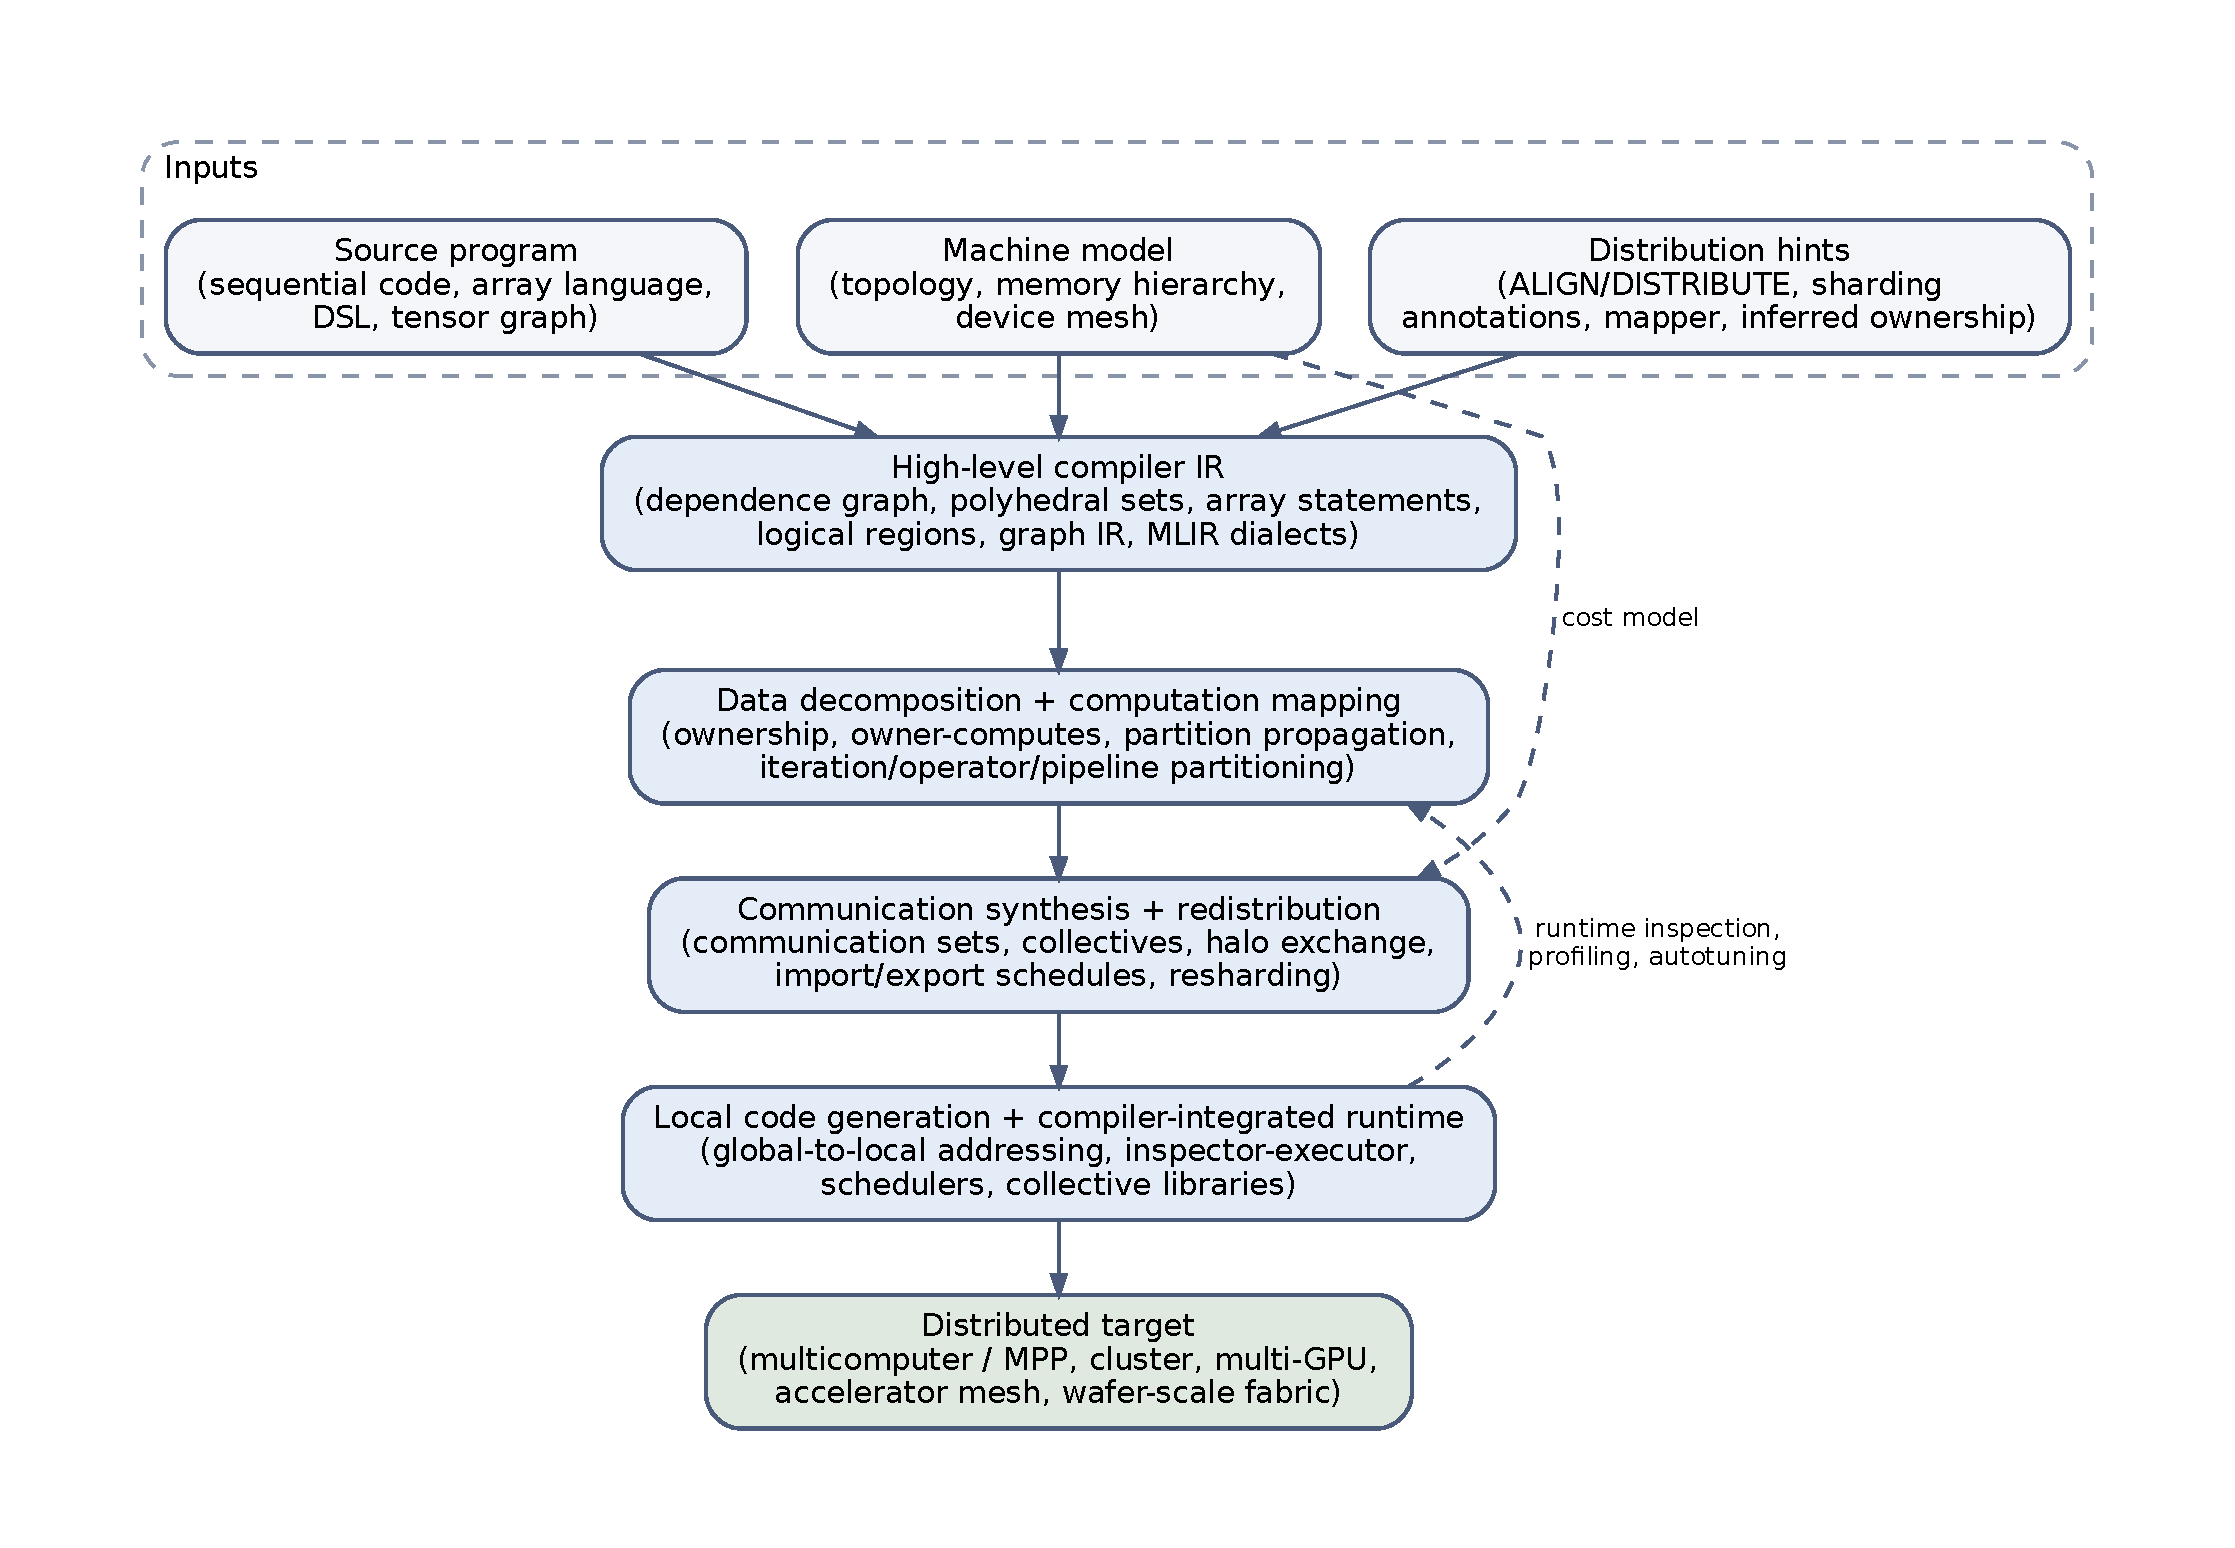
\includegraphics[width=\columnwidth]{compiler-architecture.pdf}
  \caption{The stages that recur across distributed-memory compilers from SUPERB to Shardy. The pipeline is linear in most 1990s systems; the dashed feedback edges (runtime inspection, profiling, autotuning, and cost models) are where the compiler/runtime boundary (axis~F) is drawn differently by different systems. Figure original to this survey; stages are abstracted from the catalog entries cited in the text.}
  \label{fig:architecture}
\end{figure}

\ours{We abstract the systems in the catalog into the pipeline of Fig.~\ref{fig:architecture}.} Its inputs are a source program (sequential code, an array language, a DSL, or an operator graph), a machine model (processor arrangement, device mesh, memory hierarchy, topology), and distribution information that is either supplied (ALIGN/DISTRIBUTE directives~\cite{loveman1993hpf}, sharding annotations~\cite{xu2021gspmd}, a mapper interface~\cite{bauer2012legion}) or inferred.

\paragraph{High-level IR}
\fact{Era-2 compilers worked on dependence graphs over Fortran loops~\cite{hiranandani1992compiling}; polyhedral systems represent iteration and data spaces as integer sets~\cite{bondhugula2013compiling}; ML systems use operator graphs~\cite{xu2021gspmd}; and recent work uses MLIR dialects that carry sharding or distribution attributes~\cite{bisbas2024shared,alabed2025partir}.}

\paragraph{Data decomposition and computation mapping}
\fact{The owner-computes rule, which assigns a statement to the place that owns its left-hand side, appears in the Kali and Fortran~D compilers~\cite{koelbel1991compiling,hiranandani1992compiling}; GSPMD's partition propagation infers shardings of unannotated tensors from annotated ones~\cite{xu2021gspmd}.} \infer{Both are instances of deriving a computation mapping from a data mapping; Section~\ref{sec:mapping} examines the alternatives.}

\paragraph{Communication synthesis and redistribution}
\fact{Compilers derive communication either in closed form from the distribution functions (communication sets and local address generation~\cite{koelbel1991regular,chatterjee1993generating,stichnoth1994generating}), by recognising collective patterns, or at runtime by inspecting indices~\cite{saltz1990runtime}.} Redistribution between phases is a separate stage in HPF compilers~\cite{ramaswamy1996redistribution} and reappears as resharding in SPMD partitioners.

\paragraph{Local code generation and compiler-integrated runtime}
\fact{Era-2/3 compilers emitted SPMD Fortran with calls to message-passing libraries; PARTI/CHAOS supplied runtime schedules for irregular accesses~\cite{das1994communication}; Legion executes a mapped task graph on a runtime that manages region coherence~\cite{bauer2012legion}; XLA-based systems lower to per-device programs with collective calls~\cite{xu2021gspmd}.} \ours{We use the amount of work delegated to the runtime as axis~F of the taxonomy.}

\paragraph{Synthesis}
\infer{The pipeline has been stable since the early 1990s; what has changed across eras is (i) the input abstraction, (ii) the representation on which decomposition is decided, and (iii) which stages are static versus dynamic.} These three differences are exactly axes~B, K, and F of the taxonomy.

\section{Taxonomy}
\label{sec:taxonomy}

\begin{figure}[t]
  \centering
  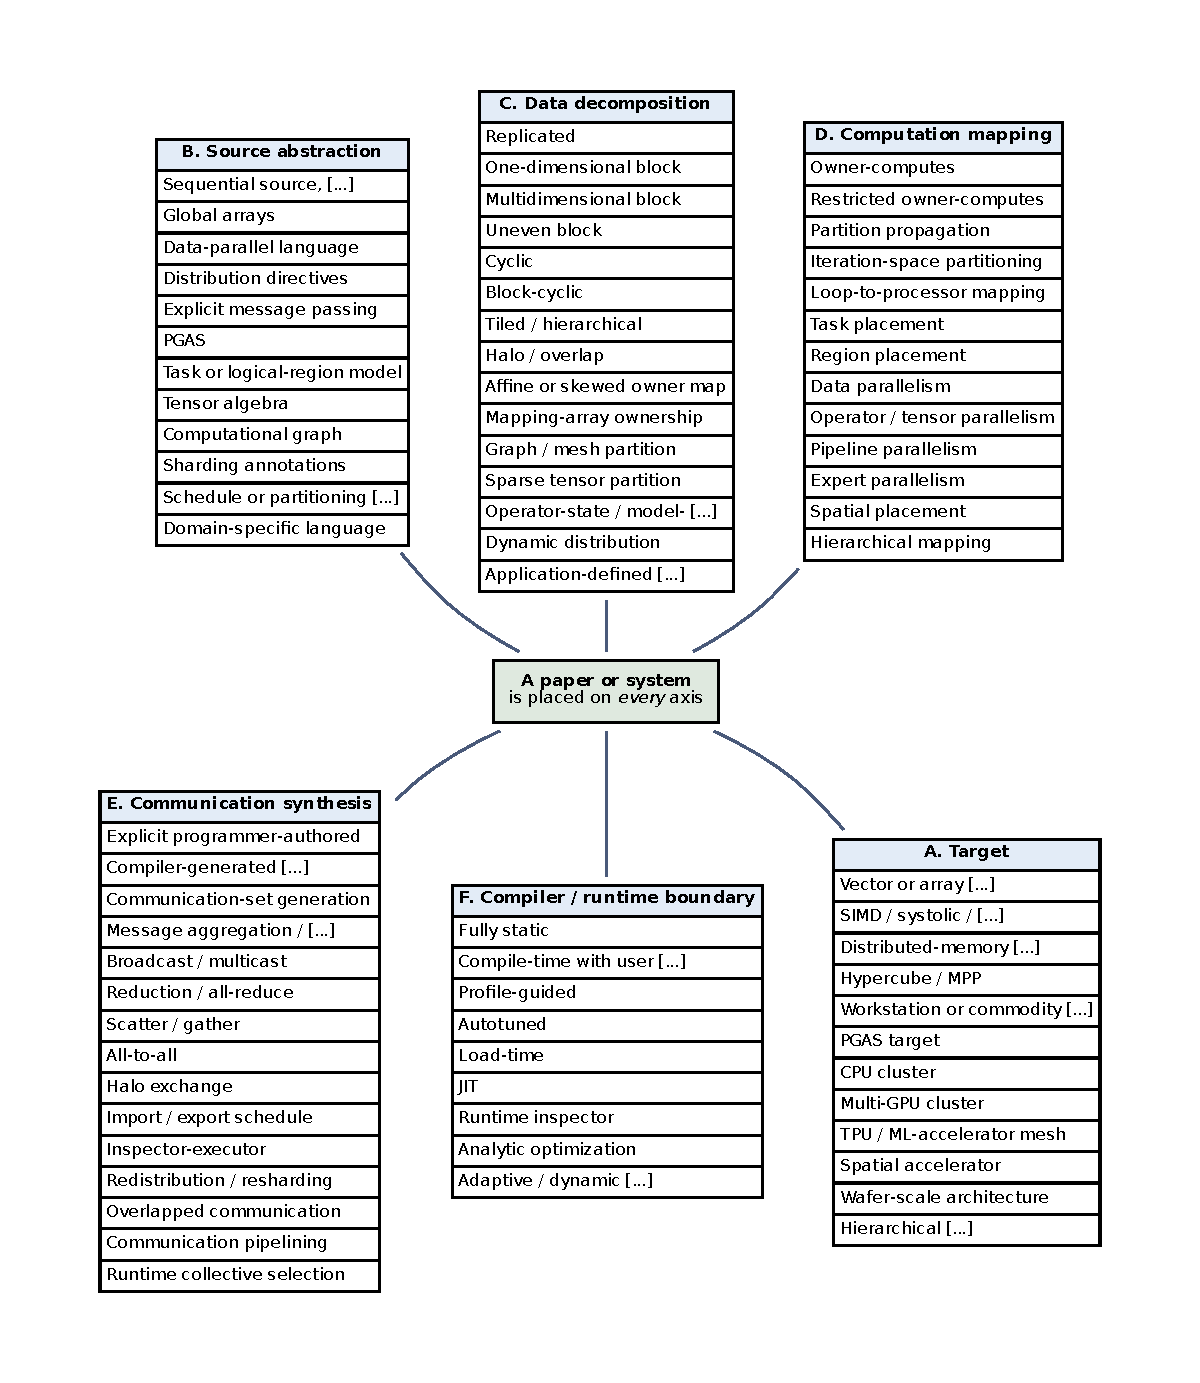
\includegraphics[width=\columnwidth]{taxonomy.pdf}
  \caption{The taxonomy is a set of orthogonal axes, not a tree: each paper or system takes one or more values on every axis. Only the six axes used most in the text are shown; the catalog carries eleven. Generated from the machine-readable taxonomy so that the figure cannot drift from the catalog.}
  \label{fig:taxonomy}
\end{figure}

\ours{We classify each paper or system along eleven independent axes (Fig.~\ref{fig:taxonomy}): (A)~target and memory model; (B)~programming abstraction (RQ1); (C)~data decomposition (RQ2); (D)~computation mapping (RQ3); (E)~communication synthesis (RQ4); (F)~compilation time, i.e. the compiler/runtime boundary (RQ5); (G)~compiler architecture; (H)~optimization objective (RQ7); (I)~maturity and artifact status; (J)~paper type; and (K)~compiler representation (RQ6).} The value lists are maintained in the repository and enforced by a validator.

\subsection{Why chronology alone is insufficient}
\infer{HPF (1993) and GSPMD (2021) take the same values on axis~C (block distribution over a logical processor grid) and on axis~E (communication inserted by propagating distributions through the program), yet they are three eras apart; inspector--executor runtimes (1990) and distributed sparse-tensor compilers (2022--2025) share the \emph{runtime inspector} value on axis~F.} A chronological list hides these recurrences, which are among the survey's main findings (Section~\ref{sec:synthesis}). Chronology is therefore one dimension (Section~\ref{sec:history}), used to explain \emph{why} a value was chosen at a given time, while the axes explain \emph{what} was chosen.

\subsection{Provenance of category names}
Where a standard term exists we use it: \emph{owner-computes} from the Kali/Fortran~D literature, \emph{inspector--executor} from PARTI, \emph{BLOCK}, \emph{CYCLIC}, and \emph{block-cyclic} from HPF, \emph{partition propagation} from GSPMD, \emph{inter-} and \emph{intra-operator parallelism} from Alpa~\cite{zheng2022alpa}. The grouping of these into axes, and the decision to place ML sharding compilers and wafer-scale compilers on the same axes as 1990s HPF compilers, is ours.

\subsection{Tagging discipline}
A tag is attached to a catalog entry only when an evidence pointer names the section of the primary source supporting it. Entries whose full text has not been consulted are tagged only on the axes their abstract clearly supports. Lineage fields record only relationships that a paper states itself or that a cited survey states; inferred lineages are kept separately. Table~\ref{tab:eras} summarises the eras, Table~\ref{tab:systems} the core systems, and Tables~\ref{tab:decomposition}--\ref{tab:evaluation} the decomposition support, compiler architecture, and evaluation methodology of each system; all are generated from the catalog.

% AUTO-GENERATED by scripts/generate_tables.py from catalog/*.yaml -- do not edit by hand.

\begin{table*}[t]
\centering
\scriptsize
\caption{Era summary. Dates are provisional (see Sec.~\ref{sec:methodology}); representative systems are the catalog entries with the highest reading priority in each era.}
\label{tab:eras}
\begin{tabular}{p{0.11\textwidth}p{0.12\textwidth}p{0.14\textwidth}p{0.14\textwidth}p{0.14\textwidth}p{0.10\textwidth}p{0.15\textwidth}}
\toprule
\textbf{Era} & \textbf{Machine driver} & \textbf{Programming abstraction} & \textbf{Decomposition representation} & \textbf{Generated communication} & \textbf{Representative systems} & \textbf{Limitation} \\
\midrule
0: Foundations (1950--1979) & Stored-program machines, FORTRAN, pipelined vector processors, lock-step array processors, dataflow and systolic proposals & Sequential FORTRAN; vector statements; early parallel-language proposals & None for distribution; dependence graphs and loop-level analysis for vectorization & None (shared or centralised memory) & -- & No notion of data placement as a compiler problem; machines had a single address space or SIMD broadcast control \\
1: Emergence of distributed-memory compilation (1980--1987) & Multicomputers and hypercubes (Cosmic Cube, iPSC, nCUBE), systolic arrays, Connection Machine & Explicit message passing; early global-array proposals; SIMD data-parallel languages & Programmer-managed; first compiler proposals for placement & Hand-written sends/receives & -- & Programming by hand was error-prone; portability across machines was poor \\
2: Global arrays and data decomposition (1988--1992) & Commercial hypercubes and MPPs (iPSC/2, iPSC/860, nCUBE-2, CM-2) & Sequential or global-array programs with distribution annotations (SUPERB, Kali, Vienna Fortran, Fortran D) & BLOCK/CYCLIC distributions, alignment to templates/decompositions, overlap regions & Compiler-generated point-to-point messages; message vectorization; first inspector-executor runtimes & \cite{callahan1988compiling,koelbel1991compiling,hiranandani1992compiling,li1991alignment} & Regular, affine programs only; automatic distribution selection intractable in general; communication costs poorly modelled \\
3: HPF, MPI, and compiler maturity (1993--2000) & MPPs (CM-5, Paragon, SP2, T3D/T3E) and early clusters & HPF directives; MPI library calls; irregular extensions; early PGAS proposals (Co-array Fortran, Titanium) at the end of the era & HPF ALIGN/DISTRIBUTE with BLOCK, CYCLIC(k), templates and processor arrangements; INDIRECT/mapping arrays in HPF-2 and research systems & Communication sets, local address generation, redistribution, collectives; PARTI/CHAOS schedules for irregular code & \cite{zima1993compiling,benkner1999compiling,banerjee1995paradigm,loveman1993hpf} & HPF compilers were slow to mature and performance was unpredictable; explicit MPI became the dominant practice \\
4: MPI dominance and alternative programming models (2000--2010) & Commodity clusters, early multicore nodes, Cell/BE and explicitly managed memories & MPI(+OpenMP); PGAS (UPC, Co-array Fortran, Titanium); HPCS languages (Chapel, X10); hierarchical memory models (Sequoia) & Language-level distributions and locales/places; hierarchical task trees & One-sided communication, compiler-scheduled bulk transfers for memory hierarchies & \cite{tang2000tiled,chen2003upc,charles2005x10,diaconescu2005reusable} & Adoption of new languages remained limited; automatic distribution rarely used in production \\
5: Compiler/runtime co-design and accelerators (2010--2019) & GPU clusters, heterogeneous nodes, early TPU pods & Affine loop nests; task/region programs (Legion, Regent); tensor DSLs; ML graph frameworks & Polyhedral partitions; logical regions and partitions; named-dimension layouts (Mesh-TensorFlow) & Polyhedral communication-set generation with MPI; dynamic region coherence; collectives in ML frameworks & \cite{bondhugula2013compiling,kruse2014molly,bondhugula2011automatic,bauer2012legion} & Each system covered one domain; no shared ownership IR; ML partitioning still largely manual \\
6: Mesh sharding, ML systems, and spatial accelerators (2020--2026) & TPU/GPU pods, AI accelerators, wafer-scale engines, spatial dataflow chips & Sharding annotations on device meshes; tensor algebra with distribution formats; MLIR dialects; stencil DSLs & Device meshes with per-dimension sharding; distributed tensor formats; MLIR shard/mesh attributes & Collective insertion by propagation; resharding; automated search over parallelism plans & \cite{xu2021gspmd,zheng2022alpa,alabed2025partir,yadav2022distal} & Dynamic/irregular workloads, heterogeneous hierarchies, and memory-capacity constraints remain weakly handled; fragmentation across frameworks \\
\bottomrule
\end{tabular}
\end{table*}

% AUTO-GENERATED by scripts/generate_tables.py from catalog/*.yaml -- do not edit by hand.

\begin{table*}[t]
\centering
\scriptsize
\caption{Core systems in the catalog. A question mark marks a cell not yet verified from a primary source.}
\label{tab:systems}
\begin{tabular}{p{0.08\textwidth}p{0.05\textwidth}p{0.06\textwidth}p{0.11\textwidth}p{0.12\textwidth}p{0.11\textwidth}p{0.12\textwidth}p{0.09\textwidth}p{0.10\textwidth}p{0.08\textwidth}}
\toprule
\textbf{System} & \textbf{Refs} & \textbf{Years} & \textbf{Input} & \textbf{Distribution} & \textbf{Work mapping} & \textbf{Communication} & \textbf{Runtime} & \textbf{Targets} & \textbf{Artifact} \\
\midrule
SUPERB & \cite{zima1988superb,gerndt1990updating} & 1986-1992 & Fortran 77 + interactive distribution & ? & ? & ? & SUPRENUM MP & SUPRENUM & unavailable \\
Kali & \cite{mehrotra1990kali,koelbel1991compiling} & 1989-1992 & Fortran + dist + doall/on & block, cyclic, block\_cyclic, user map, dynamic & on clause / owner() & in/out sets static or run-time inspector & cached inspector/executor & iPSC-class multicomputers & unavailable \\
PARTI / CHAOS & \cite{saltz1990runtime,saltz1991multiprocessor} & 1989-1997 & irregular loops with index arrays & mapping arrays via translation tables; partitioner-driven & iteration partitioning via RIG/partitioner & inspector-built import/export schedules; schedule reuse & PARTI/CHAOS & iPSC/2, iPSC/860, CM-2 & unavailable \\
Fortran D & \cite{callahan1988compiling,hiranandani1991fortrand} & 1991-1996 & Fortran 77 + decomposition directives & ? & ? & ? & NX / PARTI & iPSC/860 & unavailable \\
Vienna Fortran / VFCS & \cite{chapman1991vienna,chapman1992vienna} & 1991-1999 & Fortran 77 + DIST/ALIGN & block, cyclic(k), user-defined, INDIRECT, dynamic & owner computes; FORALL ON & overlap areas, vectorised messages (VFCS) & VFCS & iPSC/860, GENESIS, SUPRENUM & unavailable \\
PARADIGM & \cite{gupta1992automatic,su1993paradigm} & 1992-1997 & Fortran 77 (automatic) & ? & ? & ? & ? & iPSC, Paragon, CM-5 (to verify) & unavailable \\
Fortran 90D/HPF (Syracuse) & \cite{bozkus1993fortran90d} & 1993-1995 & Fortran 90D & ? & ? & runtime collective library & F90D runtime & ? & unavailable \\
High Performance Fortran (language) & \cite{loveman1993hpf,hpfforum1993spec} & 1993-2000 & Fortran 90 + directives & BLOCK, CYCLIC, CYCLIC(k), replicated; 2.0 adds INDIRECT, GEN\_BLOCK & implementation-defined (owner computes typical) & implementation-defined & n/a & n/a & specification \\
Digital (DEC) Fortran 90 HPF compiler & \cite{harris1995dechpf} & 1994-1998 & HPF 1.1 & BLOCK, CYCLIC, replicated, alignment & data-parallel; owner computes not strictly enforced & region assignments; vectorised sends; shadow edges; inlined reductions & PSE SEND/RECEIVE & Alpha workstation farms, AlphaServer SMP & commercial, unavailable \\
Titanium & \cite{yelick1998titanium} & 1998-2010 & Titanium (Java dialect) & ? & SPMD & ? & GASNet & clusters & archived \\
Co-array Fortran & \cite{numrich1998coarray} & 1998-present & Fortran + [ ] co-dimensions & one co-array per image & SPMD, programmer & explicit co-array references & ? & Cray T3E and later & spec; Fortran 2008 coarrays \\
Unified Parallel C (Berkeley UPC) & \cite{chen2003upc} & 2002-present & UPC & ? & upc\_forall affinity & ? & GASNet & clusters & open source \\
X10 & \cite{charles2005x10} & 2004-2020 & X10 & ? & at(place) / async & ? & X10RT & clusters & archived \\
Chapel & \cite{chamberlain2007chapel} & 2005-present & Chapel & user-defined domain maps (Block, Cyclic, BlockCyclic, Replicated, ...) & forall over distributed domains; on clauses & compiler + runtime (GET/PUT, aggregation) & Chapel runtime & clusters, GPUs & open source \\
Sequoia & \cite{fatahalian2006sequoia} & 2006-2010 & task trees & ? & task-to-memory-level mapping & bulk copies between levels & Sequoia runtime & Cell, clusters & unavailable \\
Pluto distributed-memory code generation (Bondhugula et al.) & \cite{bondhugula2008pluto,bondhugula2011automatic} & 2011-2016 & C affine loop nests & derived from computation partition (flow-out sets) & polyhedral iteration-space partitioning & polyhedral communication sets to MPI & MPI / dynamic scheduler & InfiniBand clusters & open source (pluto distmem branch) \\
Legion / Regent & \cite{bauer2012legion,slaughter2015regent} & 2012-present & tasks + logical regions & region partitions chosen by program/mapper & mapper interface & runtime-managed coherence and copies & Legion/Realm & GPU clusters & open source \\
Molly & \cite{kruse2014molly} & 2014-2015 & C++ + layout declarations & programmer-declared & polyhedral & generated asynchronous MPI & MPI & Blue Gene/Q (intended) & archived \\
Mesh-TensorFlow & \cite{shazeer2018meshtf} & 2018-2021 & TF graph + named dims + layout & dimension-to-mesh-axis layout & SPMD per layout & allreduce/allgather/alltoall derived from layouts & TF/TPU & TPUv2 pods & archived \\
FlexFlow & \cite{jia2019flexflow} & 2018-present & operator graph & SOAP output-tensor partitions & MCMC search with simulator & task graph with transfer tasks & FlexFlow/Legion & P100/K80 clusters & open source \\
XLA SPMD partitioner (GShard / GSPMD) & \cite{lepikhin2020gshard,xu2021gspmd} & 2020-present & HLO + sharding annotations & replicated / tiled / partially tiled per tensor over device mesh & SPMD; sharding propagation & collectives + halo exchange + resharding inserted per operator & XLA & TPUv3 pods (GPU supported) & open source (XLA) \\
Cerebras WSE programming (CSL / hand-mapped stencils) & \cite{rocki2020cerebras,jacquelin2022wse} & 2020-present & CSL & programmer-placed per-PE tiles & spatial placement & fabric colours / routes configured by programmer & SDK & CS-1/CS-2/CS-3 & commercial SDK \\
PartIR & \cite{alabed2025partir} & 2021-2025 & StableHLO + tactics & ? & ? & ? & XLA & TPU, GPU & ? \\
DISTAL / SpDISTAL & \cite{yadav2022distal,yadav2022spdistal} & 2022-2023 & tensor index notation + formats + schedule & tensor distribution notation over a processor grid; sparse non-zero/universe partitions & distribute/communicate/rotate schedule to index-task launches & Legion partitions (bounds analysis; image/preimage for sparse) & Legion & Lassen CPU/GPU nodes & open source \\
Alpa & \cite{zheng2022alpa} & 2022-2023 & JAX graph & per-stage sharding specs (ILP) & DP over stages/submeshes + ILP intra-op & GSPMD collectives + cross-mesh resharding & Alpa MPMD runtime & 64x V100 & archived \\
MLIR shard dialect (formerly mesh) & \cite{mlir2025shard} & 2023-present & MLIR + shard.grid/shard.sharding & per-axis grid sharding with halos & SPMD & all\_gather, all\_reduce, all\_to\_all, reduce\_scatter, update\_halo, send/recv & n/a & n/a & upstream MLIR \\
xDSL stencil / dmp / mpi stack & \cite{bisbas2024shared,stawinoga2026mlir} & 2023-present & stencil DSLs & static Cartesian rank-grid decomposition (dmp) & owner computes per block; one z-column per PE on WSE & dmp.swap halo exchange to mpi dialect or CSL chunked prefetch & MPI / CSL library & ARCHER2, GPUs, FPGA, CS-2/CS-3 & open source \\
Shardy (OpenXLA) & \cite{openxla2024shardy} & 2024-present & StableHLO + SDY shardings & per-axis mesh shardings & propagation & ? & XLA & TPU, GPU & open source \\
\bottomrule
\end{tabular}
\end{table*}

% AUTO-GENERATED by scripts/generate_tables.py from catalog/*.yaml -- do not edit by hand.

\begin{table}[t]
\centering
\scriptsize
\caption{Decomposition support by system. $\bullet$ supported, $\circ\!\!\bullet$ partial, $\circ$ not supported, ? not yet verified.}
\label{tab:decomposition}
\begin{tabular}{lcccccccc}
\toprule
\textbf{System} & \textbf{block} & \textbf{cyclic} & \textbf{block-cyclic} & \textbf{replication} & \textbf{halo} & \textbf{dynamic} & \textbf{irregular} & \textbf{hierarchical} \\
\midrule
SUPERB & ? & ? & ? & ? & $\textbackslash\{\}bullet$ & ? & ? & $\textbackslash\{\}circ$ \\
Kali & $\textbackslash\{\}bullet$ & $\textbackslash\{\}bullet$ & $\textbackslash\{\}bullet$ & $\textbackslash\{\}bullet$ & ? & $\textbackslash\{\}bullet$ & $\textbackslash\{\}circ\textbackslash\{\}!\textbackslash\{\}!\textbackslash\{\}bullet$ & $\textbackslash\{\}circ$ \\
PARTI / CHAOS & $\textbackslash\{\}bullet$ & $\textbackslash\{\}circ$ & $\textbackslash\{\}circ$ & $\textbackslash\{\}circ$ & $\textbackslash\{\}circ$ & $\textbackslash\{\}bullet$ & $\textbackslash\{\}bullet$ & $\textbackslash\{\}circ$ \\
Fortran D & ? & ? & ? & ? & ? & ? & ? & $\textbackslash\{\}circ$ \\
Vienna Fortran / VFCS & $\textbackslash\{\}bullet$ & $\textbackslash\{\}bullet$ & $\textbackslash\{\}bullet$ & $\textbackslash\{\}bullet$ & $\textbackslash\{\}bullet$ & $\textbackslash\{\}circ\textbackslash\{\}!\textbackslash\{\}!\textbackslash\{\}bullet$ & $\textbackslash\{\}bullet$ & $\textbackslash\{\}circ$ \\
PARADIGM & ? & ? & ? & ? & ? & $\textbackslash\{\}bullet$ & ? & $\textbackslash\{\}circ$ \\
Fortran 90D/HPF (Syracuse) & ? & ? & ? & ? & ? & ? & ? & $\textbackslash\{\}circ$ \\
High Performance Fortran (language) & $\textbackslash\{\}bullet$ & $\textbackslash\{\}bullet$ & $\textbackslash\{\}bullet$ & $\textbackslash\{\}bullet$ & $\textbackslash\{\}circ$ & $\textbackslash\{\}bullet$ & $\textbackslash\{\}circ\textbackslash\{\}!\textbackslash\{\}!\textbackslash\{\}bullet$ & $\textbackslash\{\}circ$ \\
Digital (DEC) Fortran 90 HPF compiler & $\textbackslash\{\}bullet$ & $\textbackslash\{\}bullet$ & ? & $\textbackslash\{\}bullet$ & $\textbackslash\{\}bullet$ & $\textbackslash\{\}circ$ & $\textbackslash\{\}circ\textbackslash\{\}!\textbackslash\{\}!\textbackslash\{\}bullet$ & $\textbackslash\{\}circ$ \\
Titanium & ? & ? & ? & ? & ? & ? & ? & ? \\
Co-array Fortran & $\textbackslash\{\}bullet$ & $\textbackslash\{\}circ$ & $\textbackslash\{\}circ$ & $\textbackslash\{\}bullet$ & $\textbackslash\{\}circ$ & $\textbackslash\{\}circ$ & $\textbackslash\{\}circ$ & $\textbackslash\{\}circ$ \\
Unified Parallel C (Berkeley UPC) & $\textbackslash\{\}bullet$ & $\textbackslash\{\}bullet$ & $\textbackslash\{\}bullet$ & $\textbackslash\{\}circ$ & $\textbackslash\{\}circ$ & $\textbackslash\{\}circ$ & $\textbackslash\{\}circ$ & $\textbackslash\{\}circ$ \\
X10 & ? & ? & ? & ? & ? & ? & ? & ? \\
Chapel & $\textbackslash\{\}bullet$ & $\textbackslash\{\}bullet$ & $\textbackslash\{\}bullet$ & $\textbackslash\{\}bullet$ & $\textbackslash\{\}circ\textbackslash\{\}!\textbackslash\{\}!\textbackslash\{\}bullet$ & $\textbackslash\{\}circ\textbackslash\{\}!\textbackslash\{\}!\textbackslash\{\}bullet$ & $\textbackslash\{\}circ\textbackslash\{\}!\textbackslash\{\}!\textbackslash\{\}bullet$ & $\textbackslash\{\}circ\textbackslash\{\}!\textbackslash\{\}!\textbackslash\{\}bullet$ \\
Sequoia & ? & ? & ? & ? & ? & ? & ? & $\textbackslash\{\}bullet$ \\
Pluto distributed-memory code generation (Bondhugula et al.) & $\textbackslash\{\}bullet$ & ? & ? & ? & ? & $\textbackslash\{\}circ$ & $\textbackslash\{\}circ$ & $\textbackslash\{\}circ\textbackslash\{\}!\textbackslash\{\}!\textbackslash\{\}bullet$ \\
Legion / Regent & $\textbackslash\{\}bullet$ & $\textbackslash\{\}circ\textbackslash\{\}!\textbackslash\{\}!\textbackslash\{\}bullet$ & $\textbackslash\{\}circ\textbackslash\{\}!\textbackslash\{\}!\textbackslash\{\}bullet$ & $\textbackslash\{\}bullet$ & $\textbackslash\{\}bullet$ & $\textbackslash\{\}bullet$ & $\textbackslash\{\}bullet$ & $\textbackslash\{\}bullet$ \\
Molly & $\textbackslash\{\}bullet$ & ? & ? & ? & ? & $\textbackslash\{\}circ$ & $\textbackslash\{\}circ$ & ? \\
Mesh-TensorFlow & $\textbackslash\{\}bullet$ & $\textbackslash\{\}circ$ & $\textbackslash\{\}circ$ & $\textbackslash\{\}bullet$ & $\textbackslash\{\}circ$ & $\textbackslash\{\}circ$ & $\textbackslash\{\}circ$ & $\textbackslash\{\}circ$ \\
FlexFlow & $\textbackslash\{\}bullet$ & $\textbackslash\{\}circ$ & $\textbackslash\{\}circ$ & $\textbackslash\{\}bullet$ & $\textbackslash\{\}circ$ & $\textbackslash\{\}circ$ & $\textbackslash\{\}circ$ & $\textbackslash\{\}circ$ \\
XLA SPMD partitioner (GShard / GSPMD) & $\textbackslash\{\}bullet$ & $\textbackslash\{\}circ$ & $\textbackslash\{\}circ$ & $\textbackslash\{\}bullet$ & $\textbackslash\{\}bullet$ & $\textbackslash\{\}circ$ & $\textbackslash\{\}circ$ & $\textbackslash\{\}bullet$ \\
Cerebras WSE programming (CSL / hand-mapped stencils) & $\textbackslash\{\}bullet$ & $\textbackslash\{\}circ$ & $\textbackslash\{\}circ$ & $\textbackslash\{\}circ$ & $\textbackslash\{\}bullet$ & $\textbackslash\{\}circ$ & $\textbackslash\{\}circ\textbackslash\{\}!\textbackslash\{\}!\textbackslash\{\}bullet$ & $\textbackslash\{\}circ$ \\
PartIR & ? & ? & ? & ? & ? & ? & ? & ? \\
DISTAL / SpDISTAL & $\textbackslash\{\}bullet$ & $\textbackslash\{\}circ$ & $\textbackslash\{\}circ$ & $\textbackslash\{\}bullet$ & $\textbackslash\{\}circ$ & $\textbackslash\{\}circ\textbackslash\{\}!\textbackslash\{\}!\textbackslash\{\}bullet$ & $\textbackslash\{\}bullet$ & $\textbackslash\{\}bullet$ \\
Alpa & $\textbackslash\{\}bullet$ & $\textbackslash\{\}circ$ & $\textbackslash\{\}circ$ & $\textbackslash\{\}bullet$ & $\textbackslash\{\}circ$ & $\textbackslash\{\}circ$ & $\textbackslash\{\}circ$ & $\textbackslash\{\}bullet$ \\
MLIR shard dialect (formerly mesh) & $\textbackslash\{\}bullet$ & $\textbackslash\{\}circ$ & $\textbackslash\{\}circ$ & $\textbackslash\{\}bullet$ & $\textbackslash\{\}bullet$ & $\textbackslash\{\}circ$ & $\textbackslash\{\}circ$ & $\textbackslash\{\}circ\textbackslash\{\}!\textbackslash\{\}!\textbackslash\{\}bullet$ \\
xDSL stencil / dmp / mpi stack & $\textbackslash\{\}bullet$ & $\textbackslash\{\}circ$ & $\textbackslash\{\}circ$ & $\textbackslash\{\}circ$ & $\textbackslash\{\}bullet$ & $\textbackslash\{\}circ$ & $\textbackslash\{\}circ$ & $\textbackslash\{\}circ$ \\
Shardy (OpenXLA) & $\textbackslash\{\}bullet$ & ? & ? & $\textbackslash\{\}bullet$ & ? & ? & $\textbackslash\{\}circ$ & ? \\
\bottomrule
\end{tabular}
\end{table}

% AUTO-GENERATED by scripts/generate_tables.py from catalog/*.yaml -- do not edit by hand.

\begin{table}[t]
\centering
\scriptsize
\caption{Compiler architecture by system (from catalog tags).}
\label{tab:architecture}
\begin{tabular}{lccccccp{0.3\columnwidth}}
\toprule
\textbf{System} & \textbf{src-to-src} & \textbf{polyhedral} & \textbf{graph IR} & \textbf{multi-level IR} & \textbf{MLIR} & \textbf{runtime co-design} & \textbf{Generated target} \\
\midrule
SUPERB & $\textbackslash\{\}bullet$ & $\textbackslash\{\}circ$ & $\textbackslash\{\}circ$ & $\textbackslash\{\}circ$ & $\textbackslash\{\}circ$ & $\textbackslash\{\}circ$ & Distributed-memory multicomputer \\
Kali & $\textbackslash\{\}bullet$ & $\textbackslash\{\}circ$ & $\textbackslash\{\}circ$ & $\textbackslash\{\}circ$ & $\textbackslash\{\}circ$ & $\textbackslash\{\}bullet$ & Distributed-memory multicomputer, Hypercube / MPP \\
PARTI / CHAOS & $\textbackslash\{\}circ$ & $\textbackslash\{\}circ$ & $\textbackslash\{\}circ$ & $\textbackslash\{\}circ$ & $\textbackslash\{\}circ$ & $\textbackslash\{\}bullet$ & Hypercube / MPP, Distributed-memory multicomputer \\
Fortran D & $\textbackslash\{\}bullet$ & $\textbackslash\{\}circ$ & $\textbackslash\{\}circ$ & $\textbackslash\{\}circ$ & $\textbackslash\{\}circ$ & $\textbackslash\{\}circ$ & Hypercube / MPP \\
Vienna Fortran / VFCS & $\textbackslash\{\}bullet$ & $\textbackslash\{\}circ$ & $\textbackslash\{\}circ$ & $\textbackslash\{\}circ$ & $\textbackslash\{\}circ$ & $\textbackslash\{\}circ$ & Distributed-memory multicomputer, Hypercube / MPP \\
PARADIGM & $\textbackslash\{\}bullet$ & $\textbackslash\{\}circ$ & $\textbackslash\{\}circ$ & $\textbackslash\{\}circ$ & $\textbackslash\{\}circ$ & $\textbackslash\{\}circ$ & Hypercube / MPP \\
Fortran 90D/HPF (Syracuse) & $\textbackslash\{\}bullet$ & $\textbackslash\{\}circ$ & $\textbackslash\{\}circ$ & $\textbackslash\{\}circ$ & $\textbackslash\{\}circ$ & $\textbackslash\{\}circ$ & Hypercube / MPP \\
High Performance Fortran (language) & $\textbackslash\{\}circ$ & $\textbackslash\{\}circ$ & $\textbackslash\{\}circ$ & $\textbackslash\{\}circ$ & $\textbackslash\{\}circ$ & $\textbackslash\{\}circ$ & Distributed-memory multicomputer \\
Digital (DEC) Fortran 90 HPF compiler & $\textbackslash\{\}circ$ & $\textbackslash\{\}circ$ & $\textbackslash\{\}circ$ & $\textbackslash\{\}circ$ & $\textbackslash\{\}circ$ & $\textbackslash\{\}bullet$ & Workstation or commodity cluster \\
Titanium & $\textbackslash\{\}bullet$ & $\textbackslash\{\}circ$ & $\textbackslash\{\}circ$ & $\textbackslash\{\}circ$ & $\textbackslash\{\}circ$ & $\textbackslash\{\}circ$ & PGAS target \\
Co-array Fortran & $\textbackslash\{\}circ$ & $\textbackslash\{\}circ$ & $\textbackslash\{\}circ$ & $\textbackslash\{\}circ$ & $\textbackslash\{\}circ$ & $\textbackslash\{\}circ$ & PGAS target \\
Unified Parallel C (Berkeley UPC) & $\textbackslash\{\}bullet$ & $\textbackslash\{\}circ$ & $\textbackslash\{\}circ$ & $\textbackslash\{\}circ$ & $\textbackslash\{\}circ$ & $\textbackslash\{\}circ$ & PGAS target \\
X10 & $\textbackslash\{\}bullet$ & $\textbackslash\{\}circ$ & $\textbackslash\{\}circ$ & $\textbackslash\{\}circ$ & $\textbackslash\{\}circ$ & $\textbackslash\{\}circ$ & PGAS target \\
Chapel & $\textbackslash\{\}bullet$ & $\textbackslash\{\}circ$ & $\textbackslash\{\}circ$ & $\textbackslash\{\}circ$ & $\textbackslash\{\}circ$ & $\textbackslash\{\}circ$ & PGAS target, CPU cluster, Multi-GPU cluster \\
Sequoia & $\textbackslash\{\}circ$ & $\textbackslash\{\}circ$ & $\textbackslash\{\}circ$ & $\textbackslash\{\}circ$ & $\textbackslash\{\}circ$ & $\textbackslash\{\}bullet$ & Hierarchical heterogeneous system, CPU cluster \\
Pluto distributed-memory code generation (Bondhugula et al.) & $\textbackslash\{\}bullet$ & $\textbackslash\{\}bullet$ & $\textbackslash\{\}circ$ & $\textbackslash\{\}circ$ & $\textbackslash\{\}circ$ & $\textbackslash\{\}circ$ & CPU cluster, Multi-GPU cluster \\
Legion / Regent & $\textbackslash\{\}circ$ & $\textbackslash\{\}circ$ & $\textbackslash\{\}circ$ & $\textbackslash\{\}circ$ & $\textbackslash\{\}circ$ & $\textbackslash\{\}bullet$ & Multi-GPU cluster, Hierarchical heterogeneous system, CPU cluster \\
Molly & $\textbackslash\{\}circ$ & $\textbackslash\{\}bullet$ & $\textbackslash\{\}circ$ & $\textbackslash\{\}circ$ & $\textbackslash\{\}circ$ & $\textbackslash\{\}circ$ & CPU cluster \\
Mesh-TensorFlow & $\textbackslash\{\}circ$ & $\textbackslash\{\}circ$ & $\textbackslash\{\}bullet$ & $\textbackslash\{\}circ$ & $\textbackslash\{\}circ$ & $\textbackslash\{\}circ$ & TPU / ML-accelerator mesh \\
FlexFlow & $\textbackslash\{\}circ$ & $\textbackslash\{\}circ$ & $\textbackslash\{\}bullet$ & $\textbackslash\{\}circ$ & $\textbackslash\{\}circ$ & $\textbackslash\{\}circ$ & Multi-GPU cluster \\
XLA SPMD partitioner (GShard / GSPMD) & $\textbackslash\{\}circ$ & $\textbackslash\{\}circ$ & $\textbackslash\{\}bullet$ & $\textbackslash\{\}circ$ & $\textbackslash\{\}circ$ & $\textbackslash\{\}circ$ & TPU / ML-accelerator mesh, Multi-GPU cluster \\
Cerebras WSE programming (CSL / hand-mapped stencils) & $\textbackslash\{\}circ$ & $\textbackslash\{\}circ$ & $\textbackslash\{\}circ$ & $\textbackslash\{\}circ$ & $\textbackslash\{\}circ$ & $\textbackslash\{\}circ$ & Wafer-scale architecture \\
PartIR & $\textbackslash\{\}circ$ & $\textbackslash\{\}circ$ & $\textbackslash\{\}circ$ & $\textbackslash\{\}circ$ & $\textbackslash\{\}bullet$ & $\textbackslash\{\}circ$ & TPU / ML-accelerator mesh, Multi-GPU cluster \\
DISTAL / SpDISTAL & $\textbackslash\{\}circ$ & $\textbackslash\{\}circ$ & $\textbackslash\{\}circ$ & $\textbackslash\{\}circ$ & $\textbackslash\{\}circ$ & $\textbackslash\{\}bullet$ & Multi-GPU cluster, CPU cluster \\
Alpa & $\textbackslash\{\}circ$ & $\textbackslash\{\}circ$ & $\textbackslash\{\}bullet$ & $\textbackslash\{\}circ$ & $\textbackslash\{\}circ$ & $\textbackslash\{\}circ$ & Multi-GPU cluster \\
MLIR shard dialect (formerly mesh) & $\textbackslash\{\}circ$ & $\textbackslash\{\}circ$ & $\textbackslash\{\}circ$ & $\textbackslash\{\}circ$ & $\textbackslash\{\}bullet$ & $\textbackslash\{\}circ$ & TPU / ML-accelerator mesh, Multi-GPU cluster, CPU cluster \\
xDSL stencil / dmp / mpi stack & $\textbackslash\{\}circ$ & $\textbackslash\{\}circ$ & $\textbackslash\{\}circ$ & $\textbackslash\{\}bullet$ & $\textbackslash\{\}bullet$ & $\textbackslash\{\}circ$ & CPU cluster, Multi-GPU cluster, Wafer-scale architecture \\
Shardy (OpenXLA) & $\textbackslash\{\}circ$ & $\textbackslash\{\}circ$ & $\textbackslash\{\}circ$ & $\textbackslash\{\}circ$ & $\textbackslash\{\}bullet$ & $\textbackslash\{\}circ$ & TPU / ML-accelerator mesh, Multi-GPU cluster \\
\bottomrule
\end{tabular}
\end{table}

% AUTO-GENERATED by scripts/generate_tables.py from catalog/*.yaml -- do not edit by hand.

\begin{table*}[t]
\centering
\scriptsize
\caption{Evaluation methodology by system. A question mark marks a cell not yet extracted from the primary source.}
\label{tab:evaluation}
\begin{tabular}{p{0.14\textwidth}p{0.14\textwidth}p{0.14\textwidth}p{0.14\textwidth}p{0.14\textwidth}p{0.14\textwidth}p{0.14\textwidth}}
\toprule
\textbf{System} & \textbf{Benchmarks} & \textbf{Baseline} & \textbf{Scale} & \textbf{Metrics} & \textbf{Productivity eval.} & \textbf{Artifact} \\
\midrule
SUPERB & ? & ? & ? & ? & ? & unavailable \\
Kali & ? & ? & ? & ? & ? & unavailable \\
PARTI / CHAOS & ? & ? & ? & ? & ? & unavailable \\
Fortran D & ? & ? & ? & ? & ? & unavailable \\
Vienna Fortran / VFCS & ? & ? & ? & ? & ? & unavailable \\
PARADIGM & ? & ? & ? & ? & ? & unavailable \\
Fortran 90D/HPF (Syracuse) & ? & ? & ? & ? & ? & unavailable \\
High Performance Fortran (language) & ? & ? & ? & ? & ? & specification \\
Digital (DEC) Fortran 90 HPF compiler & ? & ? & ? & ? & ? & commercial, unavailable \\
Titanium & ? & ? & ? & ? & ? & archived \\
Co-array Fortran & ? & ? & ? & ? & ? & spec; Fortran 2008 coarrays \\
Unified Parallel C (Berkeley UPC) & ? & ? & ? & ? & ? & open source \\
X10 & ? & ? & ? & ? & ? & archived \\
Chapel & ? & ? & ? & ? & ? & open source \\
Sequoia & ? & ? & ? & ? & ? & unavailable \\
Pluto distributed-memory code generation (Bondhugula et al.) & ? & ? & ? & ? & ? & open source (pluto distmem branch) \\
Legion / Regent & ? & ? & ? & ? & ? & open source \\
Molly & ? & ? & ? & ? & ? & archived \\
Mesh-TensorFlow & ? & ? & ? & ? & ? & archived \\
FlexFlow & ? & ? & ? & ? & ? & open source \\
XLA SPMD partitioner (GShard / GSPMD) & ? & ? & ? & ? & ? & open source (XLA) \\
Cerebras WSE programming (CSL / hand-mapped stencils) & ? & ? & ? & ? & ? & commercial SDK \\
PartIR & ? & ? & ? & ? & ? & ? \\
DISTAL / SpDISTAL & ? & ? & ? & ? & ? & open source \\
Alpa & ? & ? & ? & ? & ? & archived \\
MLIR shard dialect (formerly mesh) & ? & ? & ? & ? & ? & upstream MLIR \\
xDSL stencil / dmp / mpi stack & ? & ? & ? & ? & ? & open source \\
Shardy (OpenXLA) & ? & ? & ? & ? & ? & open source \\
\bottomrule
\end{tabular}
\end{table*}


\section{Historical Evolution}
\label{sec:history}

\begin{figure*}[t]
  \centering
  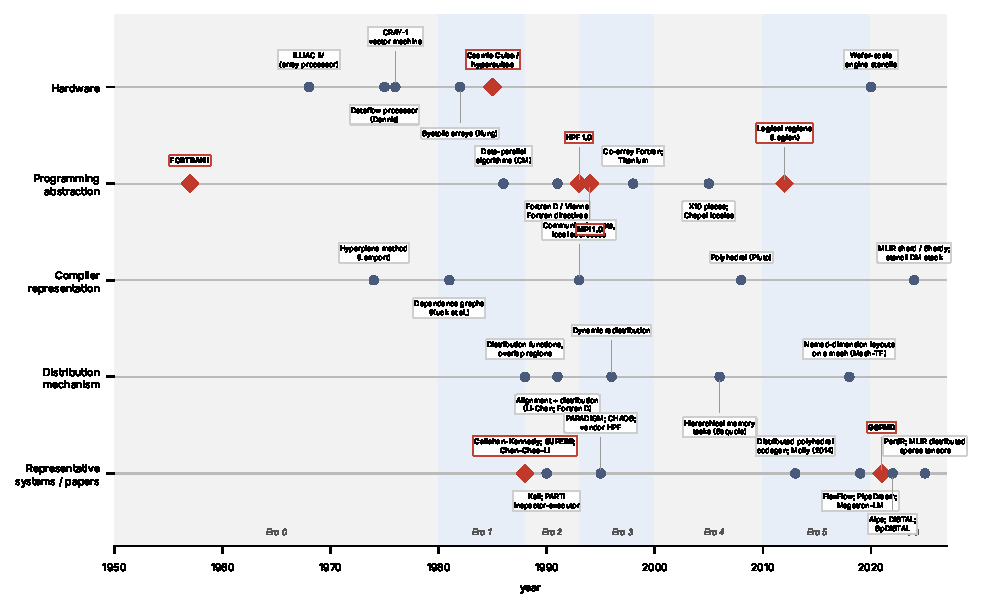
\includegraphics[width=\textwidth]{timeline.pdf}
  \caption{Timeline 1950--2026 with lanes for hardware, programming abstraction, compiler representation, distribution mechanism, and representative systems. Diamonds mark transitions that open a new era. Each event is tied to a catalog entry; era boundaries are provisional.}
  \label{fig:timeline}
\end{figure*}

Fig.~\ref{fig:timeline} and Table~\ref{tab:eras} organise the catalog into seven provisional eras. Each subsection ends with what changed, what remained, and the limitation that motivated the next era.

\subsection{Era 1: emergence (c.~1980--1987)}
\fact{Message-passing multicomputers made private memories and explicit communication the programmer's responsibility; the Cosmic Cube is the reference machine of this class~\cite{seitz1985cosmic}.} \todo{Add the early source-to-source and placement systems of this period once their records exist.}
\emph{Synthesis.} \infer{What changed: programmers faced private memories. What remained: sequential loop analysis. Limitation: all communication was hand-written, which motivated the compiler efforts of the next era.}

\subsection{Era 2: global arrays and data decomposition (c.~1988--1992)}
\fact{Zima, Bast and Gerndt's SUPERB system is described as a tool for semi-automatic MIMD/SIMD parallelisation~\cite{zima1988superb}.} \todo{Read \cite{gerndt1990updating} and state what it contributes to the handling of non-local copies in local computation.} \fact{Kali compiled global-name-space parallel loops over explicitly distributed arrays~\cite{mehrotra1990kali,koelbel1991compiling}.} \fact{Vienna Fortran extended Fortran with distribution, alignment and dynamic-distribution declarations~\cite{chapman1991vienna,chapman1992vienna}.} \fact{Fortran~D introduced decompositions and alignment with optimisations such as message vectorisation, and the 1992 evaluation measured the effect of each optimisation on an iPSC/860~\cite{hiranandani1991fortrand,hiranandani1992evaluation}.} \fact{Gupta and Banerjee chose one distribution per array by combining constraints weighted by estimated execution-time penalties~\cite{gupta1992automatic}.} \fact{Koelbel derived closed forms for communication and iteration sets of forall loops over block and cyclic arrays~\cite{koelbel1991regular}.} \fact{The PARTI runtime generated schedules for irregular loops whose access patterns are known only at run time~\cite{saltz1990runtime,saltz1991multiprocessor}.}
\emph{Synthesis.} \infer{What changed: data ownership became a compiler-visible object, and communication moved from the programmer into the compiler. What remained: dependence analysis from the foundations. Limitation: the systems handled regular affine code, and the choice of distribution was left to a costly or manual process, which motivated the standard language of the next era.}

\subsection{Era 3: HPF, MPI, and compiler maturity (c.~1993--2000)}
\fact{HPF 1.0 standardised ALIGN, DISTRIBUTE, TEMPLATE and PROCESSORS, with FORALL and INDEPENDENT~\cite{hpfforum1993spec,loveman1993hpf}.} \fact{Benkner and Zima's 1999 overview describes the compilation techniques of the decade: distribution and alignment processing, local index sets, owner-computes translation of array statements, and an inspector/executor scheme for irregular code~\cite{benkner1999compiling}.} \fact{Research compilers in this period include Fortran~90D/HPF~\cite{bozkus1993fortran90d}, PARADIGM~\cite{banerjee1995paradigm,su1995advanced} and Rogers and Pingali's Id-based compiler~\cite{rogers1994compiling}; Digital's HPF 1.1 compiler was a production product~\cite{harris1995dechpf}, and IBM's pHPF was a prototype for SP machines~\cite{gupta1995hpf}.} \fact{Closed-form communication sets for block-cyclic distributions were given by Chatterjee et al.~\cite{chatterjee1993generating}, and the redistribution problem was analysed by Ramaswamy et al.~\cite{ramaswamy1996redistribution} and Palermo et al.~\cite{palermo1996dynamic}.} \fact{MPI was standardised as the explicit alternative~\cite{mpiforum1994standard}, with MPICH as a portable implementation~\cite{gropp1996mpich}.} \fact{Kennedy, Koelbel and Zima's retrospective gives the causal account of why HPF lost most of its user base~\cite{kennedy2007rise}, and Loveman's article lists irregular and user-defined distributions among HPF's missing capabilities~\cite{loveman1993hpf}.}
\emph{Synthesis.} \infer{What changed: a standard distribution language and mature closed-form communication generation. What remained: owner-computes and block and cyclic distributions. Limitation: irregular codes were poorly served, and compiler performance was unpredictable, so practitioners used MPI directly.}

\subsection{Era 4: MPI dominance and alternative models (c.~2000--2010)}
\fact{Co-Array Fortran extends Fortran~95 with co-dimensions that name remote data by image index~\cite{numrich1998coarray}; Titanium is a Java dialect with a partitioned global address space and domain-based arrays~\cite{yelick2007titanium}; and the Berkeley UPC compiler translates UPC to C over GASNet~\cite{chen2003upc}.} \fact{Chapel presents user-definable distributions over locales as a global-view alternative to fixed directive sets~\cite{chamberlain2007chapel}.} \fact{Sequoia programs are hierarchies of tasks whose arguments describe data movement through a model of machine memory~\cite{fatahalian2006sequoia}, and Baskaran et al.\ allocate scratchpad buffers and generate movement code for explicitly managed memories~\cite{baskaran2008automatic}.} \fact{Tang and Xue generate SPMD code for rectangularly tiled, skewed iteration spaces with the computer-owns rule~\cite{tang2000tiled}.} \fact{The Pluto polyhedral optimiser~\cite{bondhugula2008pluto} provides the transformations that later distributed-memory generators build on.}
\emph{Synthesis.} \infer{What changed: distribution moved from directives into language types, domain maps and memory hierarchies. What remained: the owner concept. Limitation: adoption stayed limited, and automatic distribution was rarely used in production. \todo{Add the Berkeley UPC and HPCS evaluations, and verify the adoption claim against \cite{kennedy2007rise}.}}

\subsection{Era 5: compiler/runtime co-design and accelerators (c.~2010--2019)}
\fact{Bondhugula generated MPI communication for affine loop nests from polyhedral dependences, with flow-out and write-out sets and run-time helper functions for partners~\cite{bondhugula2011automatic,bondhugula2013compiling}; Molly does the same inside LLVM and Polly with element-level home locations~\cite{kruse2014molly}; and Dathathri et al.\ target a dataflow runtime~\cite{dathathri2014thesis,dathathri2016compiling}.} \fact{Legion expresses locality and independence with logical regions and a mapper interface~\cite{bauer2012legion}, and Regent compiles a sequential-looking language with privilege checking onto Legion~\cite{slaughter2015regent}.} \fact{Mesh-TensorFlow introduced named-dimension layouts on a processor mesh~\cite{shazeer2018meshtf}; FlexFlow searched per-operator parallelisation configurations with a simulator~\cite{jia2019flexflow}; GPipe and PipeDream established pipeline parallelism for training~\cite{huang2019gpipe,narayanan2019pipedream}; and Megatron-LM implemented tensor parallelism by hand~\cite{shoeybi2019megatron}.}
\emph{Synthesis.} \infer{What changed: accelerators and ML workloads became the driver, and representations diversified into polyhedral, region-based and mesh forms. Limitation: each system covered one domain, and the plan for an ML model was still largely a manual choice.}

\subsection{Era 6: mesh sharding, ML systems, spatial accelerators (c.~2020--2026)}
\todo{Read \cite{lepikhin2020gshard} and state its contribution from the text; it is catalogued as the predecessor of GSPMD.} \fact{GSPMD generalised annotation completion and per-operator SPMD partitioning~\cite{xu2021gspmd}. Alpa combines inter- and intra-operator parallelism~\cite{zheng2022alpa}, and PartIR composes partitioning strategies as tactics~\cite{alabed2025partir}.}
\emph{Synthesis.} \infer{What changed: the programmer writes an unpartitioned model and a mesh, and the compiler propagates the layout. Limitation: dynamic, irregular and memory-capacity-limited workloads remain weakly handled; Section~\ref{sec:open} returns to this.}

\section{Data Decomposition and Computation Mapping}
\label{sec:mapping}

\begin{figure}[t]
  \centering
  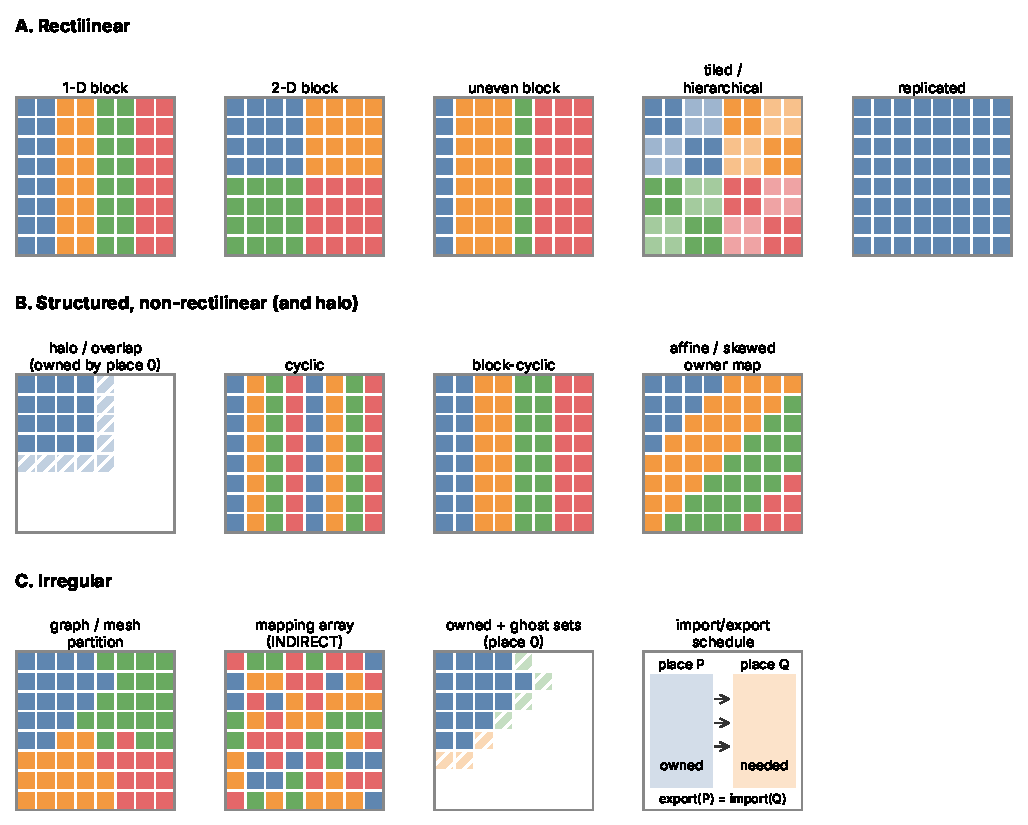
\includegraphics[width=\columnwidth]{decomposition-taxonomy.pdf}
  \caption{Data-decomposition taxonomy (axis~C) drawn as example grids coloured by owning place. Rectilinear forms (A) have closed-form owner functions. Structured non-rectilinear forms (B) need block-cyclic address arithmetic. Irregular forms (C) need a mapping array or graph partition and, usually, run-time schedules. Hatched cells are ghost copies. The examples are illustrative, not drawn from a specific system.}
  \label{fig:decomposition}
\end{figure}

\subsection{Representing ownership (RQ2)}
\ours{Fig.~\ref{fig:decomposition} groups decompositions into rectilinear, structured non-rectilinear and irregular forms.} \fact{Fortran~D and HPF express ownership by aligning arrays to a template and distributing the template over a processor arrangement, using BLOCK, CYCLIC and CYCLIC($k$)~\cite{hpfforum1993spec,loveman1993hpf}.} \fact{Koelbel and Mehrotra's Kali treats distributions as declared properties of arrays over processor arrays, and adds user-defined map functions~\cite{mehrotra1990kali}.} \fact{Vienna Fortran's distribution language includes user-defined distribution functions, alignment with linear expressions, INDIRECT mappings and dynamic redistribution with connect sets~\cite{chapman1991vienna,chapman1992vienna}.} \fact{Chatterjee et al.\ represent the local access sequence of a cyclic(k) distribution with affine alignment as a finite-state machine~\cite{chatterjee1993generating}.} \fact{Gupta and Banerjee choose one distribution per array from weighted constraints~\cite{gupta1992automatic}, and PARADIGM extends this from block to cyclic and block-cyclic distributions by symbolic partitioning~\cite{su1995advanced}.} \fact{Lee's compiler generalises the distribution function and selects layouts across consecutive loops by dynamic programming~\cite{lee1995techniques}.} \fact{Irregular ownership is expressed through a mapping array and partitioner-driven translation in CHAOS, whose partitioner can work from connectivity, coordinates or loads~\cite{ponnusamy1995runtime}.} \fact{Chandra et al.\ add regular and reshaped array distributions as directives on a cache-coherent NUMA multiprocessor, where the data layout is not a message-passing layout~\cite{chandra1997datadist}.} \fact{Modern systems express ownership as per-dimension sharding over a mesh~\cite{xu2021gspmd,mlir2025shard} or as tensor distribution formats~\cite{yadav2022distal}.}

\subsection{Assigning computation (RQ3)}
\fact{Owner-computes assigns an assignment to the owner of its left-hand side. Kali expresses it through on-clauses on doall loops~\cite{mehrotra1990kali}, and the Fortran~D compiler applies it to partition node programs~\cite{hiranandani1991fortrand}.} \fact{Koelbel's closed forms partition the iteration set of a forall loop by the same owners~\cite{koelbel1991regular}.} \fact{PARADIGM partitions iterations and data by symbolic analysis~\cite{su1995advanced} and, in the 1995 overview, combines data and functional parallelism~\cite{banerjee1995paradigm}.} \fact{Legion places tasks and regions through a mapper~\cite{bauer2012legion}, and Sequoia maps tasks to memory levels through a per-machine specification~\cite{fatahalian2006sequoia}.} \fact{ML systems choose among data, operator, pipeline and expert parallelism; Alpa chooses among them per stage with an integer program and dynamic programming~\cite{zheng2022alpa}, and FlexFlow searches per-operator partition configurations~\cite{jia2019flexflow}.}

\subsection{Synthesis}
\infer{Across these systems, the choice of computation mapping follows the choice of data mapping in most cases, and the systems differ in where the choice is made: in the programmer's directives (HPF, Kali), in a closed-form compiler analysis (Koelbel, Chatterjee), in a search over configurations (FlexFlow, Alpa), or in a mapper (Legion). \todo{Compare the expressiveness of HPF's distribution language with GSPMD sharding and DISTAL formats using the specifications \cite{hpfforum1993spec,xu2021gspmd,yadav2022distal}.}}

\section{Communication Generation and Redistribution}
\label{sec:communication}

\fact{Koelbel derived send, receive and iteration sets in closed form for forall loops over block and cyclic arrays with linear subscripts, and applied them in the Kali compiler~\cite{koelbel1991regular}.} \fact{Chatterjee et al.\ generate local addresses and communication sets for cyclic(k) distributions from a finite-state machine~\cite{chatterjee1993generating}.} \fact{Shen et al.\ revisit the Amarasinghe and Lam communication-set algorithms and remove iteration variables that do not change which element or processor is involved; on one LU kernel this reduces generated communication~\cite{shen2007eliminating,amarasinghe1993communication}.} \fact{Fortran~D's optimisations include message vectorisation for block-distributed arrays~\cite{hiranandani1991fortrand}, and the 1992 evaluation classifies them by the cost they reduce: startup, copy and transit time, or lack of parallelism~\cite{hiranandani1992evaluation}.} \fact{Tang and Xue aggregate communication per tile after skewing~\cite{tang2000tiled}.}

\subsection{Redistribution}
\fact{Ramaswamy, Simons and Banerjee represent each regular distribution as a family of line segments, so the data that must move between two processor sets is an intersection of families; they add a locality-aware packing scheme and a contention-reducing send order~\cite{ramaswamy1996redistribution}.} \fact{Palermo et al.\ extend PARADIGM's static partitioner with a recursive decomposition of a program into phases and a shortest-path search over phase transitions that accounts for redistribution cost~\cite{palermo1996dynamic}.} \fact{Lee's compiler chooses data layouts across consecutive loops by dynamic programming~\cite{lee1995techniques}.} \fact{Vienna Fortran's DISTRIBUTE statement redistributes arrays at run time~\cite{chapman1991vienna}.}

\subsection{Polyhedral and element-level generation}
\fact{Bondhugula's generator computes flow-out and write-out sets per tile, packs them, and uses compiler-generated helper functions that evaluate the processes that must receive data at run time~\cite{bondhugula2011automatic,bondhugula2013compiling}.} \fact{Molly derives asynchronous chunked MPI transfers from flow dependences, using home locations for array elements~\cite{kruse2014molly}.} \fact{Dathathri et al.\ report minimal communication volume for most dependence patterns in a dataflow runtime~\cite{dathathri2014thesis}.}

\subsection{Collectives in SPMD partitioners and tensor compilers}
\fact{GSPMD inserts collectives where propagated shardings disagree~\cite{xu2021gspmd}, and MLIR's shard dialect exposes all-gather, all-reduce, all-to-all, reduce-scatter and halo update as operations~\cite{mlir2025shard}.} \fact{Kong et al.\ restrict generated code to collectives: a cost-model constraint forbids the crossed mappings that would need point-to-point traffic, and each (operator, tensor) communication vector selects a sub-communicator~\cite{kong2023automatic}.} \fact{DISTAL expresses communication through its communicate command, and the Legion runtime realises it from partitions~\cite{yadav2022distal}.} \fact{Vaidya et al.\ implement get, set and update-slice operations over MPI all-to-all and all-to-allv~\cite{vaidya2025distributed}.}

\subsection{Halo exchange and overlap}
\fact{Bisbas et al.\ lower halo exchanges, declared in the dmp dialect, to non-blocking sends and receives in the MPI dialect; each halo is a separate exchange, and the authors note that overlap and diagonal exchanges are missing~\cite{bisbas2024shared}.} \fact{On the Cerebras engine, Stawinoga et al.\ convert halo exchanges into chunked prefetches that overlap with computation~\cite{stawinoga2026mlir}.} \fact{Rocki et al.\ overlap receiving and multiplying in background threads, while their all-reduce remains blocking~\cite{rocki2020cerebras}.}

\subsection{Synthesis}
\infer{Communication generation has moved from element-level sets, derived from affine subscripts, to collectives derived from operator semantics. The first preserves generality over index expressions; the second is simpler to model because it only needs operator-level patterns. Halo exchange has been the most stable pattern: it appears in HPF overlap areas, in SUPERB-style overlap, in the dmp dialect and in the wafer-scale runtime. \todo{Quantify the communication-volume effect of collective insertion against element-level generation using the evaluations of \cite{xu2021gspmd,alabed2025partir,kong2023automatic}.}}

\section{Runtime Analysis and Irregular Computation}
\label{sec:runtime}

\fact{Saltz and colleagues separated the work of an irregular loop into a preprocessor that builds communication pairs and translates global indices, and an executor that runs a table-driven schedule; the 1989 report measures executor overhead on an iPSC/2 at about 9--10\% for sparse matrix-vector multiplication and higher for multi-phase triangular solves~\cite{saltz1990runtime}.} \fact{The 1990 report extends this to a hashed cache and a distributed translation table, describes a prototype compiler (ARF) that generates PARTI calls for irregularly distributed arrays, and introduces the inspector and executor vocabulary~\cite{saltz1991multiprocessor}.} \fact{Das et al.\ add incremental schedules that fetch each off-processor datum once across several loops, and a mapper coupler that gives graph partitioners a runtime dependence graph~\cite{das1991irregular}.} \fact{Ponnusamy et al.\ let the user name a partitioner, and reuse inspector results when indirection arrays are unchanged, using a conservative test~\cite{ponnusamy1995runtime}; Hwang et al.\ add light-weight and two-phase schedules for adaptive irregular programs~\cite{hwang1995chaos}.} \fact{Kali's inspector results are cached and reused across repeated executions~\cite{mehrotra1990kali}.}

\fact{Rogers and Pingali combine run-time resolution, which is correct for any reference, with compile-time resolution where ownership is analysable~\cite{rogers1994compiling}.} \fact{Legion moves data-movement decisions to a runtime that reasons about logical regions and privileges~\cite{bauer2012legion}.} \fact{SpDISTAL derives ownership of sparse structures as partitions, using image and preimage operations at run time~\cite{yadav2022spdistal}.}

\subsection{Synthesis}
\infer{The runtime boundary separates systems more sharply than any other axis. Fully static, closed-form systems~\cite{koelbel1991regular,bondhugula2013compiling} are fast and predictable but restricted to affine code. Runtime-inspected systems~\cite{saltz1991multiprocessor,ponnusamy1995runtime} handle indirection at the cost of an inspector that must be amortised over repeated executions. Dynamically scheduled runtimes~\cite{bauer2012legion,dathathri2016compiling} move the decision further from the compiler. The records of Kali, PARTI and CHAOS show the same trade-off: schedule reuse is what makes the inspector affordable.}

\section{Performance Modeling and Optimization Objectives}
\label{sec:performance}

Cost models appear in the catalog in three forms: analytic models of a compiler's choices, profiles that feed a partitioner, and search over configurations scored by a simulator or a solver.

\subsection{Analytic models}
\todo{State what the performance-optimisation approach of \cite{chen1988compiling} measures, from the paper's text; the card records the Crystal language but not yet its cost model.} \fact{Gupta and Banerjee weight distribution constraints by estimated execution-time penalties, and note that the combined problem is NP-hard and that their estimates rest on compile-time assumptions about loop bounds and branch probabilities~\cite{gupta1992automatic}.} \fact{Palermo et al.\ describe their static pipeline cost model as conservative~\cite{palermo1996dynamic}.} \fact{Kong et al.\ minimise local work plus a weighted communication volume under per-node memory capacity; their cost model is volume-only, without latency or bandwidth terms, and the paper reports no numeric speedups in its text~\cite{kong2023automatic}.}

\subsection{Profiles and simulators}
\fact{PipeDream's optimiser uses a single-GPU profile of per-layer compute time, activation size and parameter size, and a dynamic program over a hierarchical bandwidth model that minimises the time of the slowest stage~\cite{narayanan2019pipedream}.} \fact{FlexFlow's simulator profiles each operator once and re-simulates incrementally during a Markov-chain search over per-operator configurations; the authors state that the simulator assumes operator times are predictable and independent of input data~\cite{jia2019flexflow}.}

\subsection{Search and hierarchical optimisation}
\fact{Alpa solves intra-operator parallelism with an integer program over enumerated algorithms with resharding costs, and inter-operator parallelism with dynamic programming over profiled stage costs~\cite{zheng2022alpa}.} \fact{PartIR's automatic tactic uses an analytical simulator and Monte Carlo tree search, and the propagation itself uses no cost heuristics~\cite{alabed2025partir}.}

\subsection{Objectives}
\ours{Table-free summary of axis~H as the catalog records it. Communication volume is the objective of the analytic and search systems above~\cite{kong2023automatic,jia2019flexflow}; load balance and pipeline stage time dominate the training planners~\cite{narayanan2019pipedream,zheng2022alpa}; local memory fit is the constraint in~\cite{kong2023automatic} and the motivation for model-state sharding in~\cite{rajbhandari2020zero}; and productivity is the claimed benefit of the declarative systems~\cite{shazeer2018meshtf,alabed2025partir}.} \todo{Tabulate the objective of each core system with evidence pointers once all cards are merged; the catalog currently carries the tags but not the comparison.}

\subsection{Synthesis}
\infer{Analytic models were abandoned for automatic distribution in the 1990s, and the modern systems that search do so over operator-level choices, where profiling is cheap. \todo{Test this against the records of Gupta and Banerjee and Palermo et al.\ before stating it as a finding.}}

\section{Multi-GPU, ML, Spatial, and AI-Accelerator Compilers}
\label{sec:modern}

\fact{Mesh-TensorFlow expresses a program as named tensor dimensions mapped onto a mesh of processors, so any dimension can be split and the collectives follow from the layouts~\cite{shazeer2018meshtf}.} \fact{GSPMD completes sharding annotations by priority-based propagation and partitions every operator, covering data, model, spatial and pipeline parallelism through one mechanism~\cite{xu2021gspmd}.} \fact{Its authors report 50--62\% TPUv3 utilisation on up to 2048 cores and models with up to one trillion parameters, without a cost model or search~\cite{xu2021gspmd}.} \fact{PartIR separates partitioning tactics from the model and composes them on an MLIR-based IR~\cite{alabed2025partir}.} \fact{OpenXLA's Shardy combines the GSPMD and PartIR approaches~\cite{openxla2024shardy}, and the MLIR shard dialect, formerly called mesh, is described as inspired by GSPMD~\cite{mlir2025shard}.}

\fact{Automatic search is represented by FlexFlow~\cite{jia2019flexflow} and Alpa~\cite{zheng2022alpa}. Pipeline training is represented by PipeDream, which partitions layers into stages from a profile and schedules them with weight stashing~\cite{narayanan2019pipedream}, and by GPipe~\cite{huang2019gpipe}. Megatron-LM implements tensor parallelism by hand~\cite{shoeybi2019megatron}, and ZeRO is catalogued for model-state sharding~\cite{rajbhandari2020zero}; its card is pending. We classify the last four as bridge entries because their plan generation is manual or limited.}

\fact{DISTAL and SpDISTAL bring distribution formats and scheduling commands to dense and sparse tensor algebra, compiled to Legion~\cite{yadav2022distal,yadav2022spdistal}. Kong et al.\ derive distributed-memory mappings for tensor DAGs automatically~\cite{kong2023automatic}. Vaidya et al.\ express distributed sparse tensors as an MLIR dialect that lowers to MPI~\cite{vaidya2025distributed}.}

\fact{On spatial and wafer-scale targets, Rocki et al.\ hand-map a BiCGStab solver onto the Cerebras engine with one mesh column per core and a hardware-routed AllReduce~\cite{rocki2020cerebras}; Jacquelin et al.\ study scalable distributed high-order stencil computations~\cite{jacquelin2022wse} (the machine and results are pending a read of the paper); and Stawinoga et al.\ compile stencil DSLs to the Cerebras software language through three new dialects~\cite{stawinoga2026mlir}.} \fact{Bisbas et al.\ give stencil DSLs distributed-memory parallelism on clusters through a shared stack~\cite{bisbas2024shared}.}

\todo{Add a card for Tiramisu~\cite{baghdadi2019tiramisu}, which the catalog lists with distributed-memory support, and for the 2024 Shardy and MLIR documentation once read in full. The accelerator-vendor compilers named in the brief (Graphcore, SambaNova, Tenstorrent, Groq) are not yet catalogued.}

\section{Cross-Era Synthesis}
\label{sec:synthesis}

\begin{figure*}[t]
  \centering
  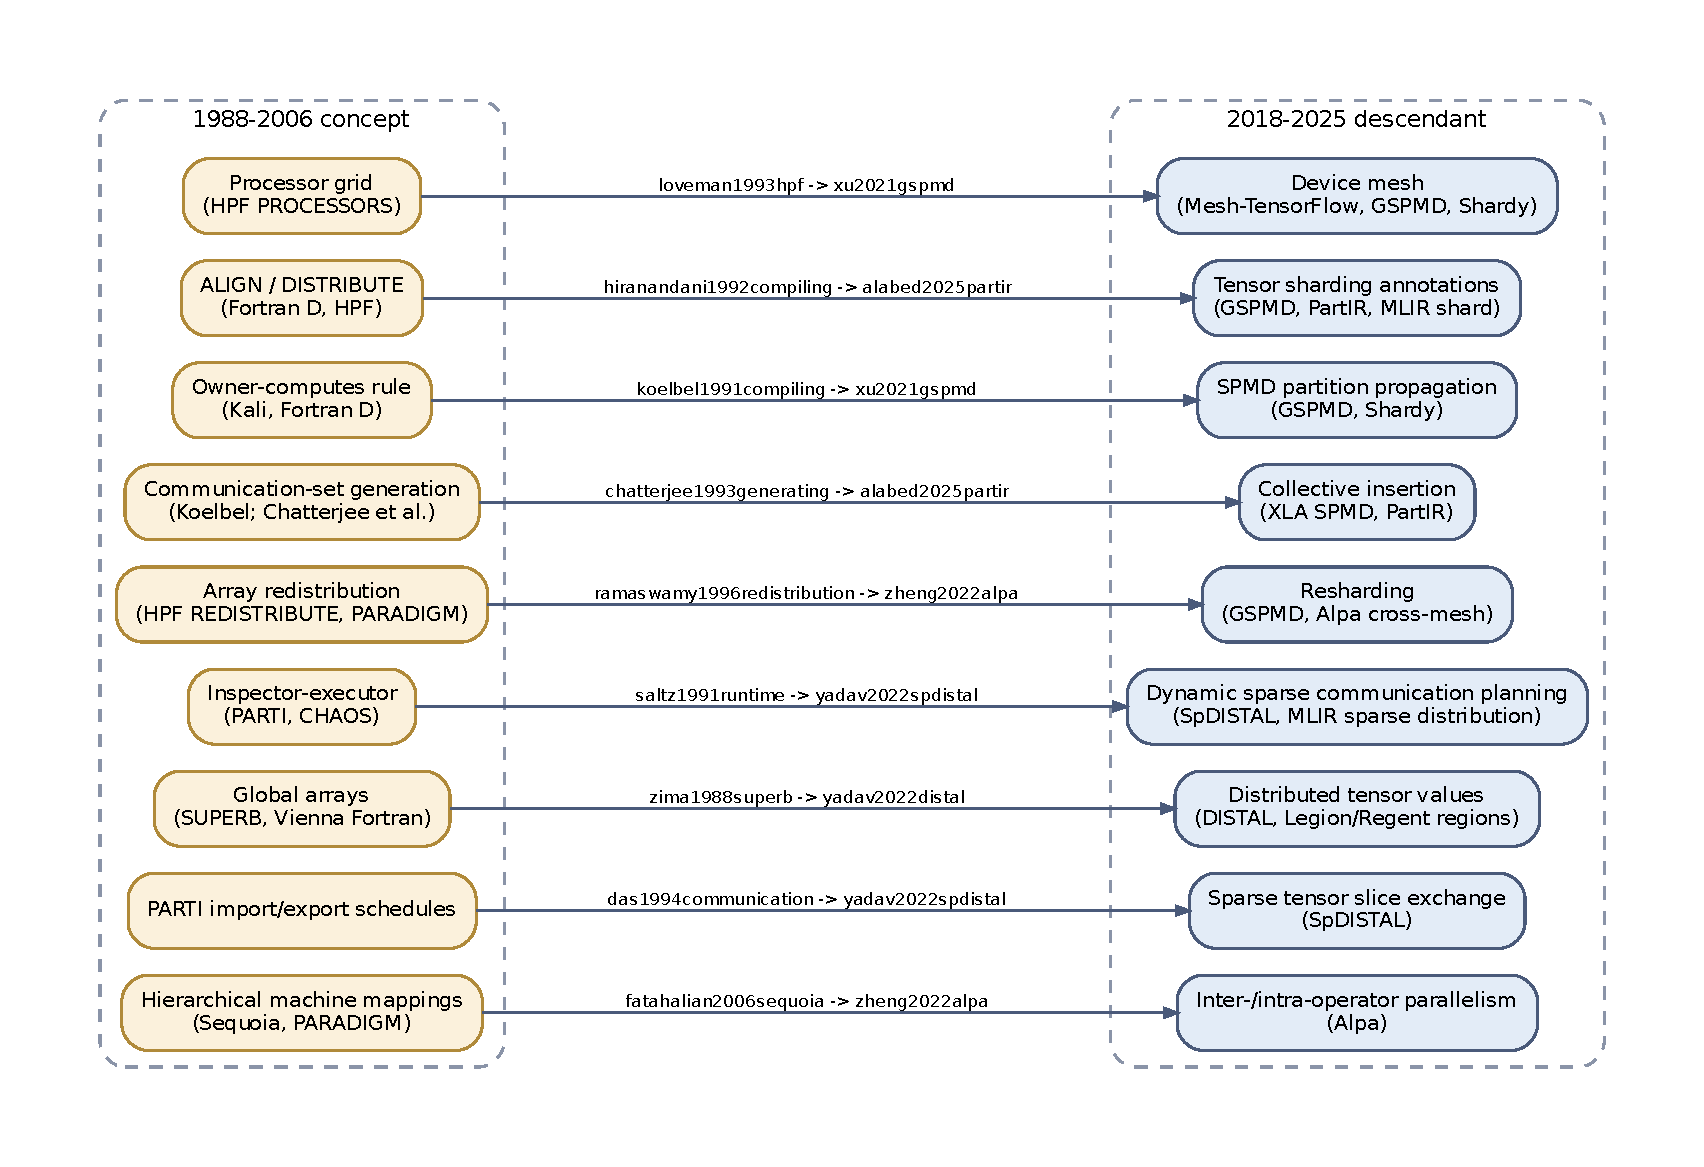
\includegraphics[width=0.9\textwidth]{rediscovery-map.pdf}
  \caption{Concepts of 1988--2006 and their 2018--2025 descendants. Each edge names the catalog entries that document the older and the newer form. The pairing is a survey hypothesis: it asserts functional correspondence, not that the newer work cites the older one; evidence for each pair is tracked in the repository's historical-claims file.}
  \label{fig:rediscovery}
\end{figure*}

\subsection{Ideas that persisted}
\infer{Logical processor grids, block distributions, owner-derived computation mapping, and the separation of a global index space from local storage persisted from Era~2 through Era~6 (Fig.~\ref{fig:rediscovery}).}

\subsection{Ideas that failed or receded}
\infer{Fully automatic distribution selection for general Fortran programs receded after Era~3; the HPF retrospective attributes HPF's decline to immature compilers, unpredictable performance, and missing support for irregular codes~\cite{kennedy2007rise}.} \todo{Confirm the attribution against the text of \cite{kennedy2007rise} and \cite{benkner1999compiling}.}

\subsection{Concepts rediscovered under new names}
\infer{Processor grid $\rightarrow$ device mesh; ALIGN/DISTRIBUTE $\rightarrow$ sharding annotation; owner-computes $\rightarrow$ partition propagation; communication sets $\rightarrow$ collective insertion; redistribution $\rightarrow$ resharding; inspector--executor $\rightarrow$ dynamic sparse communication planning; global arrays $\rightarrow$ distributed tensor values; PARTI import/export $\rightarrow$ sparse slice exchange; hierarchical machine mapping $\rightarrow$ inter-/intra-operator parallelism.}

\subsection{Why explicit MPI became dominant, and why high-level partitioning has returned}
\infer{We hypothesise that MPI won in Era~3--4 because its cost model is transparent to the programmer and its performance does not depend on compiler maturity, whereas high-level partitioning has returned in Era~6 because ML programs are expressed as operator graphs with few, large, regular operators, which makes both propagation and cost modelling tractable in a way that general Fortran loops were not.} \todo{Test this hypothesis against the evaluation sections of \cite{xu2021gspmd,zheng2022alpa,alabed2025partir} and against \cite{kennedy2007rise}.}

\section{Open Problems}
\label{sec:open}

Each problem below follows from a generalization in Table~\ref{tab:generalizations} and names the evidence that would close it.

\begin{itemize}[leftmargin=*,nosep]
  \item \textbf{Measured versus modelled cost (G2).} No read paper compares a network model against a profile on one workload. Until one does, the shift from analytic to measured optimisation is an explanation, not a result~\cite{gupta1992automatic,jia2019flexflow}.
  \item \textbf{Unified ownership and layout IR (G1, G7).} Closed-form owners, declared maps and propagated shardings need different analyses. The MLIR shard dialect is the nearest candidate for a shared representation, and the sparse dialect of Vaidya et al.\ is a second~\cite{mlir2025shard,vaidya2025distributed}.
  \item \textbf{Propagation under constraints.} PartIR's authors report that propagation is blocked by reshapes and non-divisible shapes~\cite{alabed2025partir}; GSPMD's sharding completion is heuristic~\cite{xu2021gspmd}. The conditions under which propagation is unique are not characterised.
  \item \textbf{Overlap of reductions.} Halo exchanges overlap with computation, but among the read papers we did not find a reduction overlapped with the computation that feeds it~\cite{bisbas2024shared,rocki2020cerebras}.
  \item \textbf{Break-even of run-time stages.} No read paper reports when an inspector pays for itself against a fully static schedule~\cite{saltz1990runtime,ponnusamy1995runtime}.
  \item \textbf{Correctness of generated communication.} Verification is rarely addressed. The PartIR core is the exception, with a lowering that its authors report as proved~\cite{alabed2025partir}.
  \item \textbf{Wafer-scale and fine-grained memory.} Both read wafer-scale compilers keep the decomposition static and one tile per processing element, and the stencil runtime supports only star-shaped patterns~\cite{stawinoga2026mlir,rocki2020cerebras}.
  \item \textbf{Productivity.} Productivity is recorded as an objective for five to seven of the ten Era~6 papers, depending on the coding, but none of the read papers measures it with users~\cite{xu2021gspmd,alabed2025partir}.
\end{itemize}
\todo{Each item needs its test from Table~\ref{tab:generalizations} run, or an explicit statement that it was not run.}

\section{Conclusion}
\label{sec:conclusion}

Distributed-memory compilation has been revisited for each new class of machine with private memories. The early systems of the late 1980s and 1990s made ownership a compiler-visible object, and HPF standardised a declarative distribution language that did not survive as a user-facing standard. Explicit MPI and PGAS languages carried the field through the 2000s. The current wave expresses distribution as sharding over meshes, with partitioning propagated by the compiler. The catalog, taxonomy and figures are maintained openly so that each new wave can begin from the records of the last rather than from scratch. \todo{Finalise once the remaining cards are merged and the cross-era hypotheses are tested.}


\bibliographystyle{IEEEtran}
\bibliography{../bibliography/references}

\end{document}
